\documentclass[draft]{agujournal2019}

\newcommand{\todo}[1]{\textcolor{red}{\textbf{(#1)}}}

\usepackage{amsmath}

\linenumbers
\journalname{Journal of Advances in Modeling Earth Systems (JAMES)}

\begin{document}

\title{Responses to Humidity and Temperature Perturbations in High-Resolution Simulations of Convection}

\authors{Timothy H. Raupach\affil{1,2}, Chimene L. Daleu\affil{3}, Robert S.
Plant\affil{3}, Steven S.Sherwood\affil{1,2}, and Yi-Ling Hwong\affil{4}}

\affiliation{1}{Climate Change Research Centre, University of New South Wales, Sydney, Australia}
\affiliation{2}{ARC Centre of Excellence for Climate Extremes}
\affiliation{3}{Department of Meteorology, University of Reading, Reading, United Kingdom}
\affiliation{4}{Institute of Science and Technology Austria, Vienna, Austria}

\correspondingauthor{Timothy H. Raupach}{timothy.h.raupach@gmail.com}

\begin{keypoints}
\item \todo{1-3 key points, $\leq$ 140 characters each}
\end{keypoints}

\begin{abstract}
\todo{Abstract\ldots}
\end{abstract}

\section*{Plain Language Summary}
\todo{Plain language summary\ldots}

\section{Introduction}

In the atmosphere, deep convection refers to overturning circulations formed by
bouyant air that reach the tropopause \cite{Wallace_2006}. Deep convection is
responsible for the formation of the most severe thunderstorms \todo{ref}. While
deep convection covers only a small proportion of the Earth's surface at any one
time, its resulting storms produce a large proportion of the Earth's rainfall
\cite{Wallace_2006}. Deep convection also warms the atmosphere and balances
radiative cooling, such that on average the tropics remain in
radiative-convective equilibrium (RCE) \cite{Manabe_JAS_1964}. These important
effects mean that models such as global and regional climate models
(respectively GCMs and RCMs) need to take deep convection into account. However,
models often use horizontal grid spacings that are much larger than the
horizontal scale of convection, meaning that they are unable to resolve
individual convective cells. In this case, the model must account for the
effects of convection -- such as its heating effect or rain it may produce -- by
parameterising the sub-grid convection that it can not explicitly resolve. Such
parameterisations are called convection schemes. 

Many different convection schemes have been produced, each with different
strengths, weaknesses, and assumptions \todo{On convection schemes, see Arakawa
2004, Kain and Fritsch 1990, Rio 2019}. Such are the differences between these
schemes that convection parameterisation is a leading source of uncertainty in
model outputs \cite{Hwong_JAMES_2021} \todo{other refs}. It is difficult to
compare convection schemes, since traditional methods in which simulated outputs
are compared with observations \todo{many from pg. 2 in Hwong 2021} rely on
observation selection and accuracy \cite{Hwong_JAMES_2021} \todo{Emmanul 1994}.

The mathematical framework proposed by \citeA{Kuang_JAS_2010} uses linear
response functions to compare model behaviour via assessment of the models'
responses to small perturbations in the larger-scale atmospheric properties. In
this method, the responses of the model (and thus the convection scheme) are
examined in idealised simulations under different small perturbations to the
humidity and temperature tendencies. The idea is that although there are many
non-linear processes in convection, the statistics of the cumulous ensemble as a
whole can be well-described by smooth linear functions that describe how the
ensemble reacts to small changes in its large-scale environment
\cite{Kuang_JAS_2010}. An advantage of this approach is that the responses of
the model to perturbations can be distilled by the linear response functions,
which describe the model behaviour well enough to, for example, describe the
dynamics of convectively coupled waves \cite{Kuang_JAS_2010}. Even if a linear
approximation is inadequate for fully describing convection, it can be a useful
first-order characterization.

The linear response framework was applied to single column models (SCMs) by
\citeA{Herman_JAMES_2013} \todo{specifically for the purpose of testing a couple
of convection schemes}. \citeA{Hwong_JAMES_2021} used the framework to evaluate
convection, planetary boundary, and microphysics schemes' responses to
perturbations in SCMs. They showed that the results isolate the convection
scheme in at least the tested SCMs, and examined a large number of schemes in
actual use \cite{Hwong_JAMES_2021}. The technique allows for efficient
comparison of different model setups, but does not answer the question of which
setup is most accurate. To answer this question study of the linear responses of
a model that uses the fewest possible parameterisations is required.
\citeA{Kuang_JAS_2010} performed a large ensemble of large eddy simulation (LES)
runs, but used a rather coarse resolution of 4 km and only a single LES model
(SAM \todo{write in full}).

Here, we ran perturbation experiments on models at high resolution and compared
the results to perturbations run at lower resolution, to attempt to produce
benchmark results and determine the effect of the planetary boundary layer (PBL)
scheme when convection is resolved explicitly. The key question is whether the
response of a cloud-resolving model (CRM) or large eddy simulation (LES) to a
forcing perturbation is robust, or whether it is sensitive to modelling
decisions that one might make in high-resolution modelling, such as the grid
length, model dynamics, or the microphysics used. A related question is whether
the response is dominated by the modelled convection itself, or whether it might
be sensitive to the specification of surface properties in an idealized
modelling setting. All this is important in being able to judge differences
between models in \citeA{Hwong_JAMES_2021}. Do differences seen between models
point to errors in one or more convection parameterizations, or are they within
the uncertainties found in different credible LES simulations? The rest of this
manuscript is organised as follows. In Section \ref{sec:methods} we introduce
the methods we used including modelling setups. Results are shown in Section
\ref{sec:results} and conclusions are drawn in Section \ref{sec:conclusions}.

\section{Methods}
\label{sec:methods}

We used two models in this work: the Advanced Research (AR) version of the
Weather Research and Forecasting (WRF) model, version 4.1.4
\cite{Skamarock_2019}, and the Met Office/NERC Cloud Model (MONC) \todo{version,
reference}. 

\subsection{Common Model Settings}

Both models were used to simulate convection at high resolution over
a water surface with periodic boundary conditions. The models used a constant
sea surface temperature (SST) of 301.15 K. This value is a little different from
that used in \citeA{Kuang_JAS_2010} but matches \citeA{Hwong_JAMES_2021}.

Radiative cooling and evaporation were both idealised. We used idealised
radiation as in \citeA{Herman_JAMES_2013} and \citeA{Hwong_JAMES_2021}, but
unlike \citeA{Kuang_JAS_2010} who used interactive radiation. Following
\citeA{Herman_JAMES_2013}, the radiative cooling tendency was $\theta_{tend,rad}
= \theta_t/\Pi$ K day$^{-1}$, where $\Pi$ is the Exner function that converts
temperature to potential temperature, and $\theta_t$ is a temperature tendency
set as \todo{double check in code for both WRF and MONC}

\begin{align}
 \theta_t = \begin{cases}
    -1.5\; \textrm{K day}^{-1} & \textrm{if}\, p \geq 200\; \textrm{hPa}, \\
    0\; \textrm{K day}^{-1} & \textrm{if}\, p \leq 100\; \textrm{hPa}, \\
    -1.5 + \frac{1.5 (p-100)}{100}\; \textrm{K day}^{-1} & \textrm{if}\, 100 < p < 200\; \textrm{hPa}. \\
 %* $t$'s value varies linearly between -1.5 and 0 K day$^{-1}$ from 100 to 200 hPa.
 \end{cases}
\end{align}

We used idealised evaporation as in \citeA{Chua_GRL_2019} with minor
differences. We used a constant surface wind speed of $W_s = 4.8$ m s$^{-1}$,
following \citeA{Hwong_JAMES_2021} who used the same approach with a fixed value
of 0.001 for the surface exchange coefficients. While the wind speed here and in
\citeA{Hwong_JAMES_2021} was slightly different from that of
\citeA{Kuang_JAS_2010}, the important quantity is the product of the wind with
the surface exchange coefficient, and the exchange coefficient value in
\citeA{Kuang_JAS_2010} was not stated.

Horizontal winds were relaxed to 0 m s$^{-1}$ with a four-day relation time.
\todo{By level-mean wind or pixel-by-pixel?} \todo{Is this true for both WRF and
MONC? Different for 1 km (Chimene) runs in WRF.}.

For each resolution, the models were run until they reached radiative convective
equilibrium (RCE) at time $t_1$. After RCE was reached, small perturbations in
temperature or moisture fields were introduced, while a control was run with no
perturbations, and the models were allowed to again reach RCE at time $t_2$.
Domain-mean atmospheric profiles for time $t_1$ were subtracted from those at
$t_2$ to examine the differences made by the perturbations. In the following two
sections we examine the model-specific setups for WRF and MONC, respectively.

\subsection{WRF}

WRF was run on a 20 $\times$ 20 km$^2$ domain for horizontal grid spacings of 4
km, 1 km and 100 m. The runs at 4 km and 1 km grid resolution used 74 grid
points in the vertical while the run at 100 m grid spacing used 370 grid points
in the vertical. The parameterisations used are summarised in Table
\ref{tab:WRF_schemes}. The model timestep was set to 6 s for 4 km and 1 km grid
spacing and 1 s for 100 m grid spacing, and outputs were recorded hourly in all
cases. For the runs with 1 km and 4 km grid spacing, the models were initialised
using a Radiative-Convective Equilibrium Model Intercomparison Project (RCEMIP)
profile \cite{Wing_GMD_2018}. For the runs at 100 m grid spacing, the model was
initialised using the RCE model state from the 1 km runs, to start close to RCE
and reduce computation time. Temperature and water vapour mixing ratio in the
stratosphere were relaxed to the initial profile values to avoid model drift, as
suggested by \citeA{Herman_JAMES_2013}. Relaxation was applied above 160 hPa
with the inverse relaxation constant increasing linearly from $1/\tau = 0$
day$^{-1}$ at 160 hPa to $1/\tau = 0.5$ day$^{-1}$ at and above 100 hPa
\cite{Herman_JAMES_2013}. Full diffusion (\texttt{diff\_opt = 2}) was used at
all resolutions; at 4 km and 1 km resolutions, horizontal diffusion was
diagnosed from deformation and vertical diffusion was assumed done by the
planetary boundary layer scheme (\texttt{km\_opt = 4}) while the simulations at
100 m used a prognostic equation (\texttt{km\_opt = 3}) for turbulent kinetic
energy \cite{Skamarock_2019}.

\begin{table}[t]
    \caption{Parameterisations used in the WRF simulations. These schemes were
     used for all resolutions, with the exception of the boundary layer scheme
     which was enabled only for the 4 km and 1 km simulations. No convection
     parameterisation was used.}
    \label{tab:WRF_schemes}
    \centering
    \begin{tabular}{lll}
    \hline
    \textbf{Parameterisation} & \textbf{Scheme} & \textbf{Reference} \\
    \hline
    Microphysics & Thompson & \citeA{Thompson_MWR_2008} \\
    Boundary layer & YSU & \citeA{Hong_MWR_2006} \\
    Surface layer & Revised MM5 & \citeA{Jimenez_MWR_2012} \\
    Land surface & Thermal diffusion & \citeA{Dudhia_1996} \\
    \hline
    % \multicolumn{2}{l}{$^{a}$Footnote text here.}
    \end{tabular}
\end{table}

We used idealised evaporation as in \citeA{Chua_GRL_2019} and
\citeA{Hwong_JAMES_2021}, with a fixed surface wind speed and the drag
coefficient assumed to be 0.001. Then surface heat flux (SH) was calculated
using modified Eq. 1 from \citeA{Chua_GRL_2019}, such that

$$
\textrm{SH} = 0.001 \rho_a W c_p (T_s - T_a),
$$

\noindent where $\rho_a$ (kg m$^{-3}$) is the near surface air density, $T_s$
(K) is surface temperature (we use SST), and $T_a$ (K) is the near-surface air
temperature. We used 

$$
T_a = T_l \left(\frac{p_s}{p_l}\right)^{\frac{R_d}{c_p}},
$$

\noindent where $T_l$ (K) is the temperature at the first model level above the
surface, $p_s$ (hPa) is surface pressure, $p_l$ (hPa) is pressure at the first
model level, $c_p$ (J kg$^{-1}$ K$^{-1}$) is the specific heat capacity of dry
air at constant pressure, and $R_d$ (J kg$^{-1}$ K$^{-1}$) is the gas constant
for dry air. Latent heat flux (LH) was calculated using modified Eq. 2 from
\citeA{Chua_GRL_2019}, such that

$$
\textrm{LH} = 0.001 \rho_a W L (q_{sat} - q_a),
$$

\noindent where $L$ is the typical latent heat of vaporization of water,
$q_{sat}$ is the saturated water vapour mixing ratio at $T_s$ (we use WRF's
``ground saturated mixing ratio'') and $q_a$ is the water vapour mixing ratio at
the lowest model level. Note that while \citeA{Chua_GRL_2019} assumed that air
density near the surface is 1 kg m$^{-3}$, we used the near-surface density
value produced by WRF (around 1.16 kg m$^{-3}$).

Because the pressure levels in the WRF model were not exactly at the points
around which we want to perturb, we adapted the form of perturbations used by
\citeA{Herman_JAMES_2013} so that only the Gaussian portion of the perturbation
function is used, and instead of selecting a level $k$ a pressure $p_p$ (hPa)
around which to perturb is selected. The perturbation function used in the WRF
simulations for the $i$th model level was

$$
f_i = \exp\left[ - \left( \frac{p_p - p_i}{75 \textrm{hPa}}\right)^2 \right],
$$

\noindent where $p_p$ (hPa) is the chosen perturbation pressure and $p_i$ is the
pressure at level $i$.

We calculated the spatial means per interpolated model pressure level, per time
step. The average of these mean profiles over the RCE period was calculated for
each run for comparison.

\subsection{MONC}

MONC was run on a \todo{X $\times$ X km$^2$} domain for grid spacings of 1 km
and 500 m. We used an idealized treatment of evaporation in the sense that a
constant surface wind speed was imposed. However, the surface exchange
coefficient was calculated by the MONC model itself. The mean value calculated
was a little larger than that in \citeA{Chua_GRL_2019}, with the product of the
exchange coefficient and the surface wind speed being $5.2 \times 10^{-3}$ m
s$^{-1}$ in the MONC simulations compared with $5 \times 10^{-3}$ m s$^{-1}$ for
the fixed Chua parameters. \todo{MONC settings including parameterisations
used.}

\begin{itemize}
    \item \todo{BP: On 02/12/21 and 09/12/21 and beyond, there was a change of design to match
    the idealized treatment of evaporation with WRF -- check which version we are
    showing results from here.}    
    \item \todo{BP: A change in the treatment of surface fluxes was made on
    11/05/22. I believe the setup remained fixed after this date and so that is
    what we should publish. However, there may be a question about showing results
    at the three resolutions if they are only available for this first setup?}
    \item \todo{BP: The idealized treatment of evaporation as in Chua et al (2019) was
    altered to match with the MONC simulations. i.e., with the near surface wind of
    5 ms-1 rather than 4.8.}
    \item \todo{BP: I believe we stuck with this value (TR: ie of surface wind
    speed? I think the WRF sims use 4.8 ms-1) which makes our setup slightly
    different from Hwong et al (2021). That's a little unfortunate, but I don't
    suggest to rerun but simply to note that this made very little difference.}
    \item \todo{BP: Other minor changes were made in the relaxation to mean winds to
    match between the two models, but again these did not have any significant
    effects on the results.}
    \end{itemize}

\section{Results}
\label{sec:results}

\subsection{Radiative-Convective Equilibrium Mean State}

We used plots of spatially-averaged precipitable water by time to determine when
the models had reached RCE. Figure \ref{fig:rce_pw} shows precipitable
water by time for the runs. For the WRF runs, at 4 km grid spacing the RCE state
had a precipitable water (PW) of $\sim$37 mm, which rose to $\sim$42 mm at 1 km
grid spacing and $\sim$41 mm at 100 m grid spacing.

\begin{figure}[pth]
    \noindent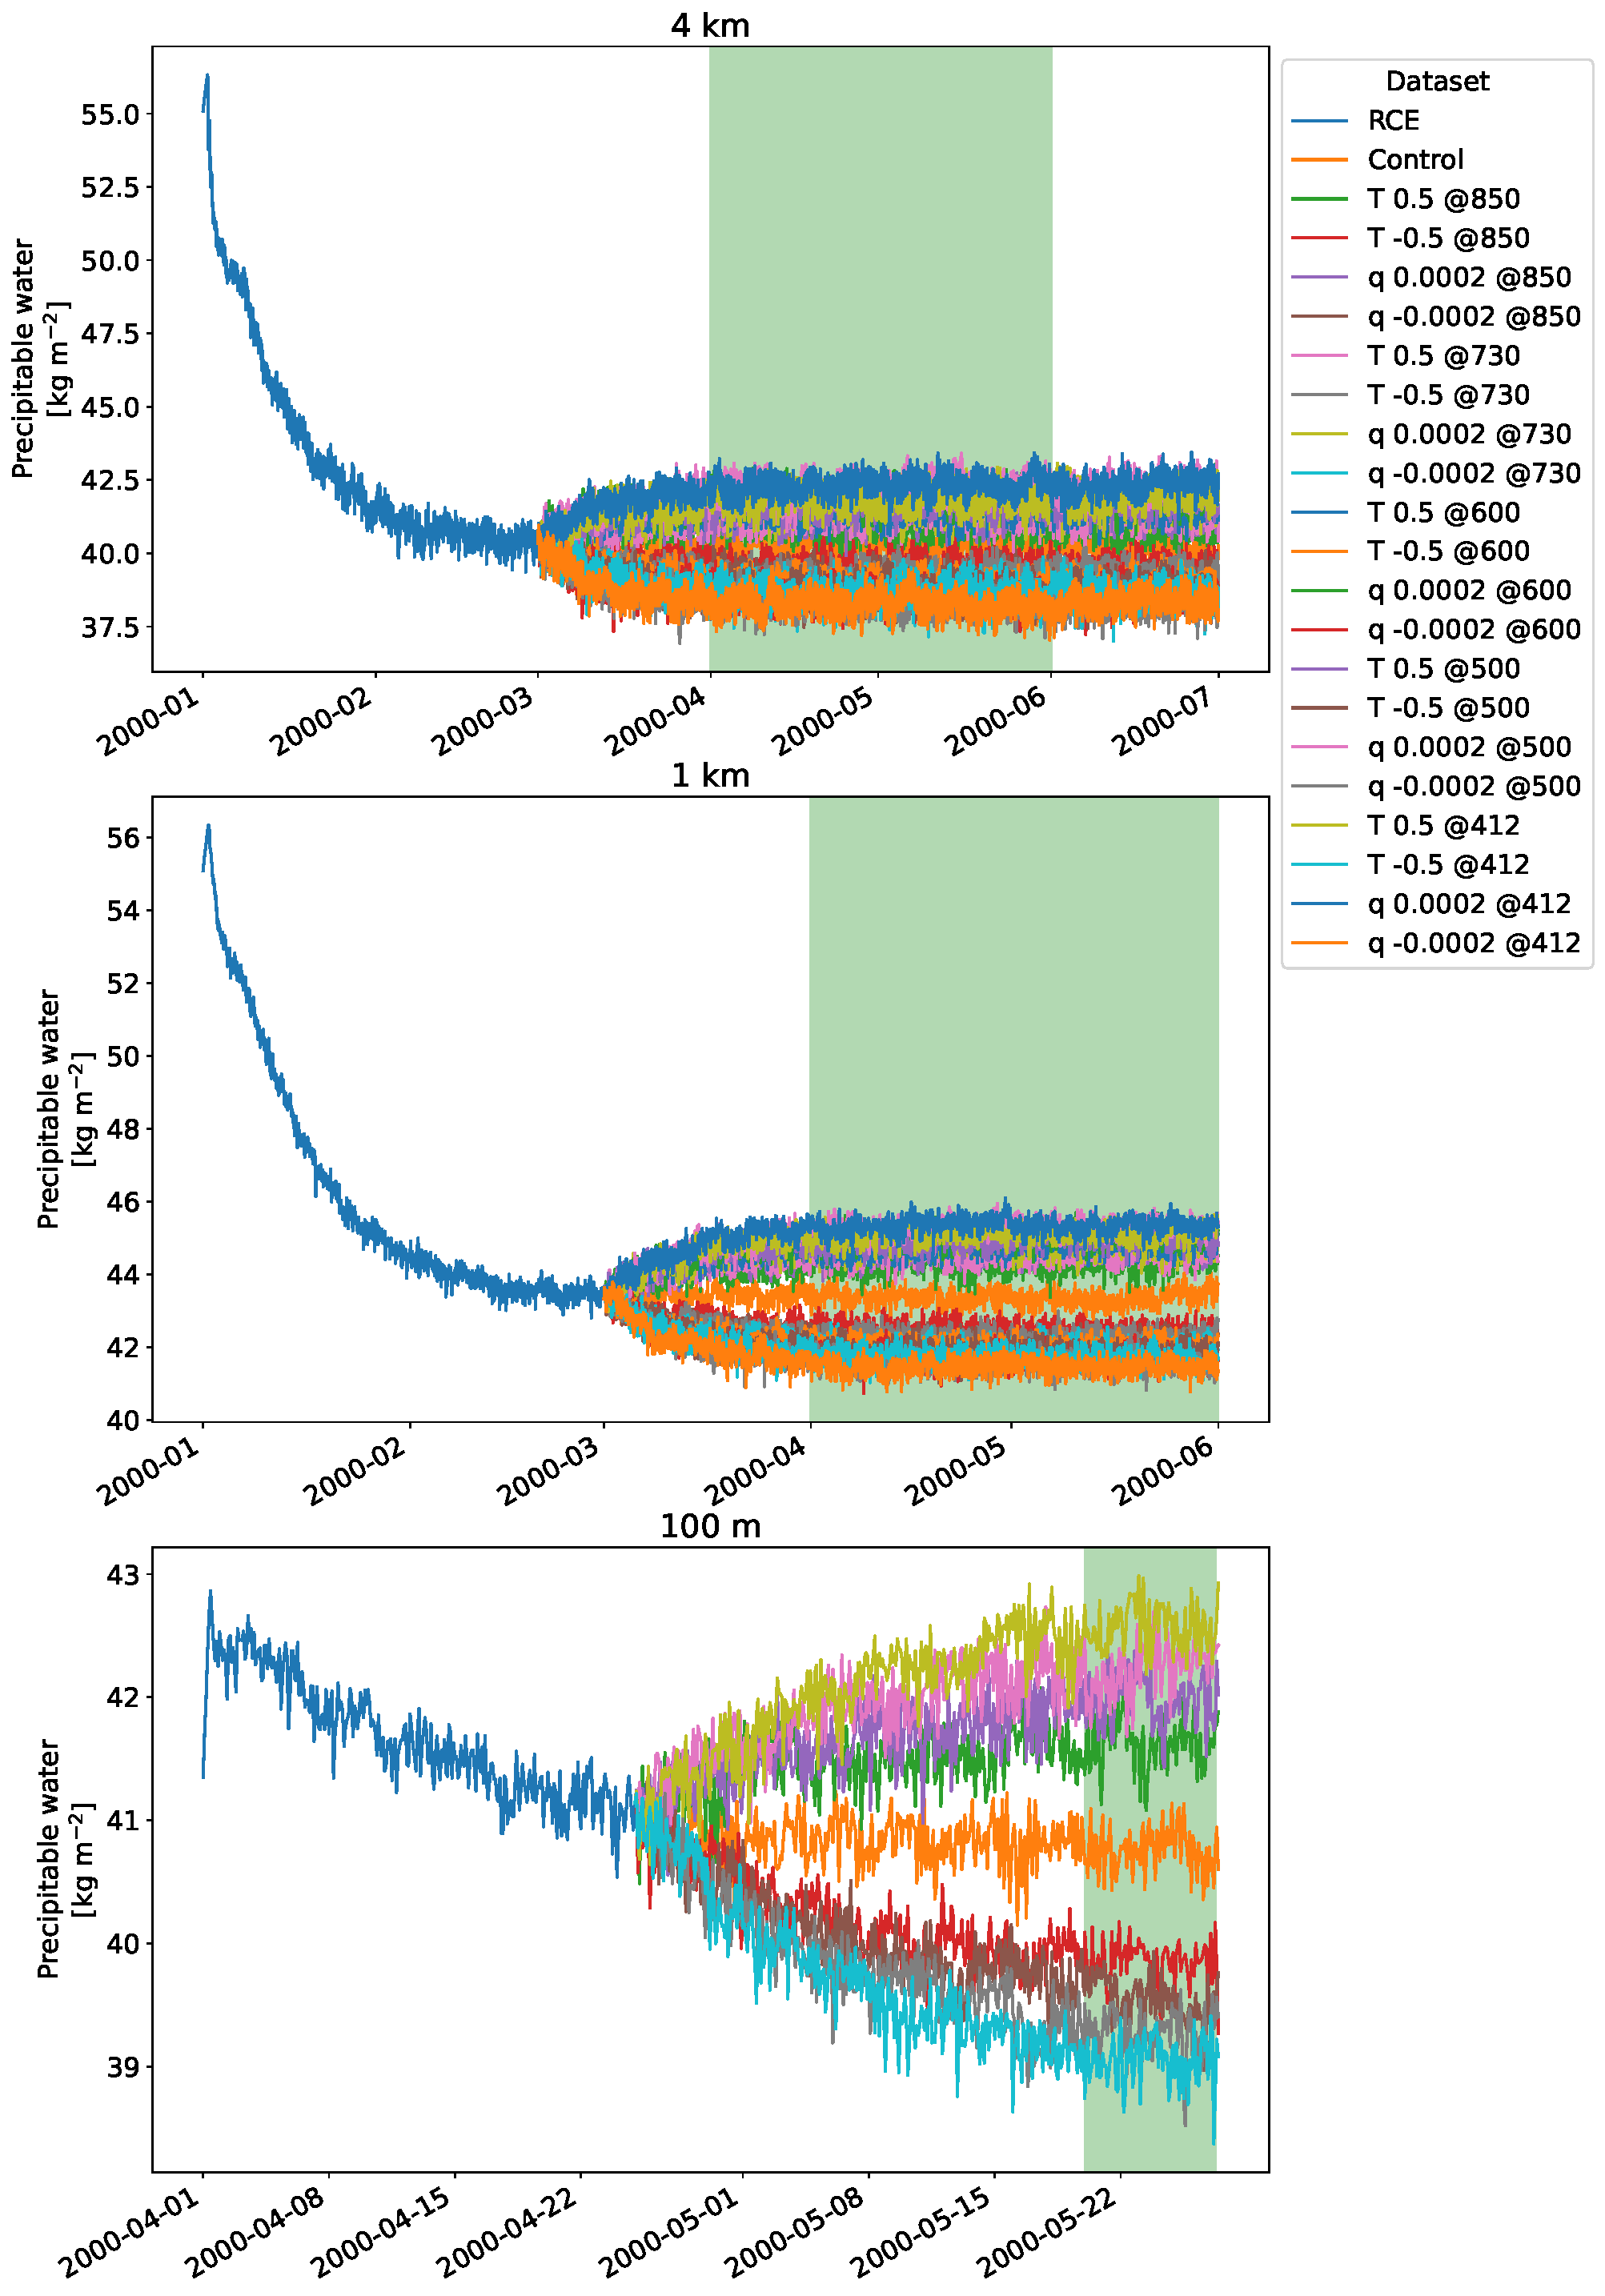
\includegraphics[width=\textwidth]{figures/RCE_PW} \caption{Spatial
    mean precipitation water produced by the WRF model by grid spacing and time.
    The RCE run was computed until mean precipitable water stabilised and the
    model was at RCE. At this point the perturbations were introduced and the
    model was run until all perturbed runs were also at RCE. The parts of the
    time axes highlighted in green show the ``RCE region'' over which mean
    profiles were calculated for comparison. \todo{Include MONC results?}}
    \label{fig:rce_pw}
\end{figure}

Mean profiles from the control run in RCE are shown in Figure
\ref{fig:rce_profiles}. \todo{The mean states are fairly similar across the two
models -- certainly within the context of larger inter-model comparisons of RCE
states (examples?), although to some extent the similarities may be due to the
idealised treatment of radiation and evaporation used here}. Moisture content
increases with increasing resolution, although the changes are modest at 1 km
and higher-resolution grid spacing. \todo{MONC is perhaps marginally more moist
than WRF.} The additional moisture at finer resolutions appears in the lower
part of the free troposphere, which we hypothesise is the result of some
transport from shallow convection. Mean wind profiles for the 100 m run, which
had increased vertical resolution than, and was temporally shorter than the
other runs, are not as smooth as those for the 1 km and 4 km runs. At 100 m grid
spacing the profile of relative humidity is fairly uniform with height between
$\sim$950 and $\sim$600 hPa, whereas at 1 km and 4 km grid spacing this part of
the atmosphere was drier, with the 4 km grid spacing simulation drying to
$\sim$60\% relative humidity at about 800 hPa.

\begin{figure}[pth]
    \noindent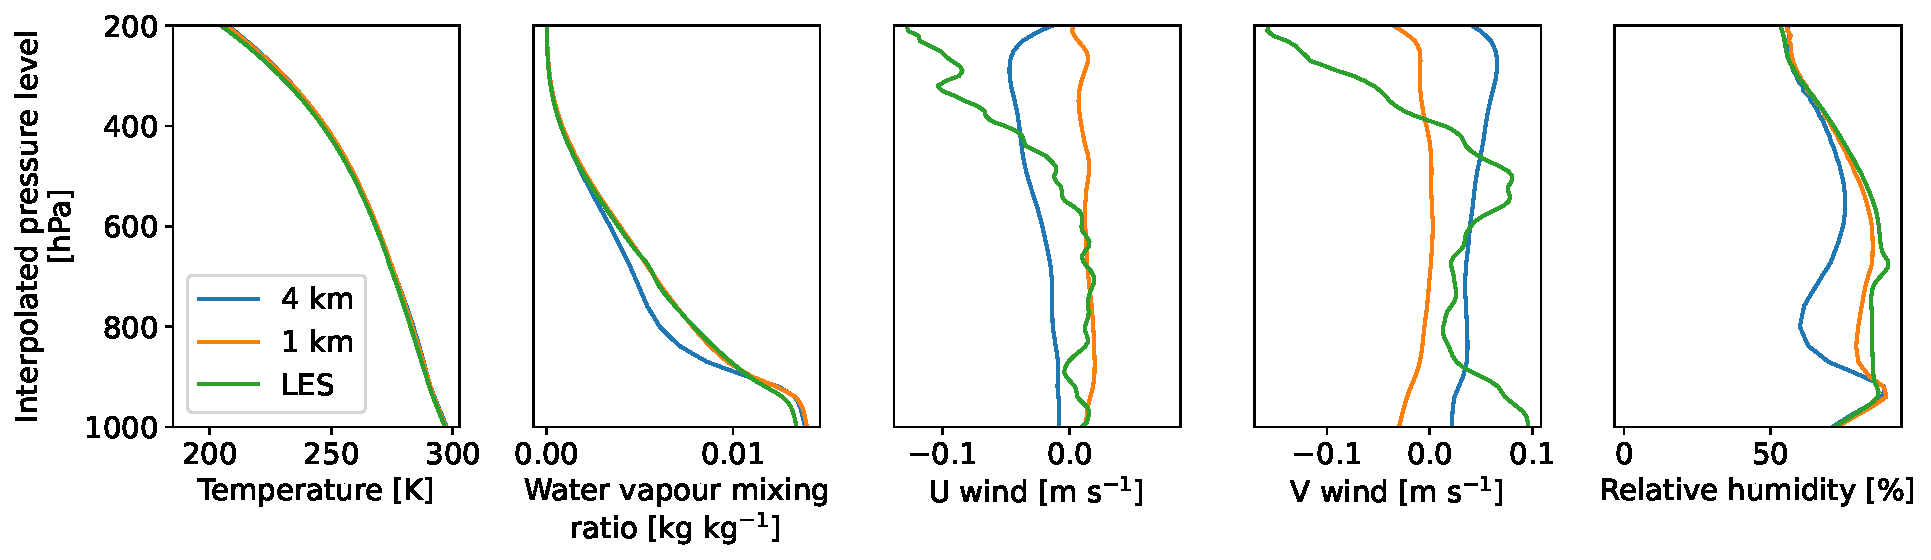
\includegraphics[width=\textwidth]{figures/RCE_profiles}
    \caption{Mean profiles for selected variables in the control runs' RCE
    periods, by grid spacing. \todo{Include MONC results on the same plots.}}
    \label{fig:rce_profiles}
\end{figure}

Mean profiles for hydrometeor classes are shown in Figure
\ref{fig:rce_hydrometeors}. Hydrometeor profiles are sensitive to resolution in
WRF, with increasing resolution resulting in more rain below $\sim$650 hPa and
less rain above, increases in cloud droplets and snow particles. There were
mixed changes for ice and graupel content. There is less sensitivity in changes
with resolution in MONC, but the character of the changes is broadly the same --
we note that the MONC results are missing the large resolution change between 4
km and 1 km that is shown in the WRF results. The sharp difference between WRF's
cloud droplet mixing ratio at 1 km compared with 100 m grid spacing does not
have a counterpart in the MONC results. In both models we see an increase in ice
content at cloud top, and in both models there is less graupel at high
resolution, with relative differences varying by height. It is hard to say if
these microphysics changes may be simply a reflection of there being more
moisture in the mean state with resolution or whether they reflect changes in
the representation of clouds. Profile shapes seem broadly similar between WRF
and MONC, with perhaps the strongest difference in liquid water for which MONC
has significantly more at $\sim$800 hPa and less above $\sim$600 hPa. Graupel
and snow are found at lower heights in WRF than in MONC.

\begin{figure}[pth]
    \noindent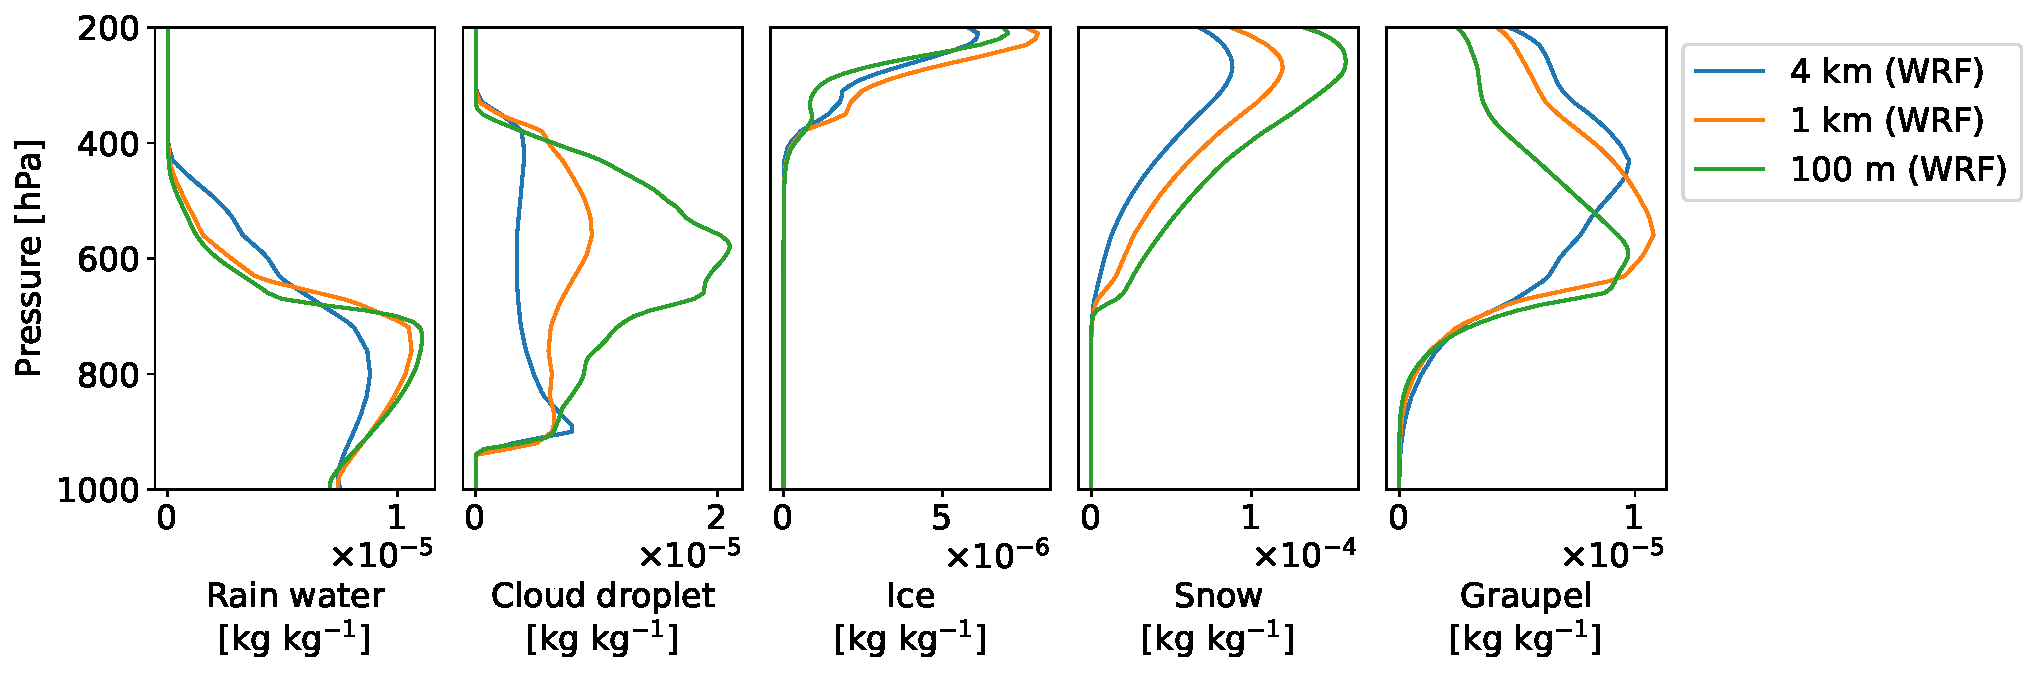
\includegraphics[width=\textwidth]{figures/RCE_hydrometeors}
    \caption{Mean profiles for hydrometeor concentrations in the control runs'
    RCE periods, by grid spacing. All values are mixing ratios.
    \todo{Include MONC results on the same plots.}}
    \label{fig:rce_hydrometeors}
\end{figure}

\subsection{Convective Organisation}

We tested for convective organisation by examining the spatial variance of
precipitable water scaled by its spatial mean (not shown), and found no evidence
of meaningful organisation in these fixed-radiation setups.

\subsection{Responses to Perturbations in Temperature}

The responses of the models to perturbations in temperature at 412 hPa, 500 hPa,
600 hPa, 730 hPa, and 850 hPa are shown in Figures \ref{fig:tpert_412},
\ref{fig:tpert_500}, \ref{fig:tpert_600}, \ref{fig:tpert_730}, and
\ref{fig:tpert_850}, respectively. In all cases, the moisture and hydrometeor
responses to forcing perturbations are much smaller than the changes in the mean
profiles due to resolution (Figures \ref{fig:rce_profiles} and
\ref{fig:rce_hydrometeors}). WRF and MONC produce responses of similar
amplitude. MONC is more likely to show nonlinearity to positive and negative
perturbations than WRF \todo{not certain, given missing MONC negative
perturbation profiles in the current results}, with the strongest example being
the temperature response in the upper troposphere to a temperature perturbation
at 850 hPa. 

\begin{itemize}
   \item \todo{Bob: WRF has been run for positive and negative perturbations at
   both 500m and 1km. There is  little indication of nonlinearity in WRF for the
   temperature and moisture responses, but the 500m run does show some marked
   nonlinearity in the hydrometeor response, specifically for rain water, for
   liquid water at upper levels and for graupel.}
   \item \todo{Tim: WRF was run at 4 km, 1 km and 100 m - do you mean MONC at
   500 m or WRF at a different resolution?}
   \item \todo{Steve: need to check whether discrepancies are actually
   non-linearity or just noise.}
\end{itemize}

\begin{figure}[pth]
    \noindent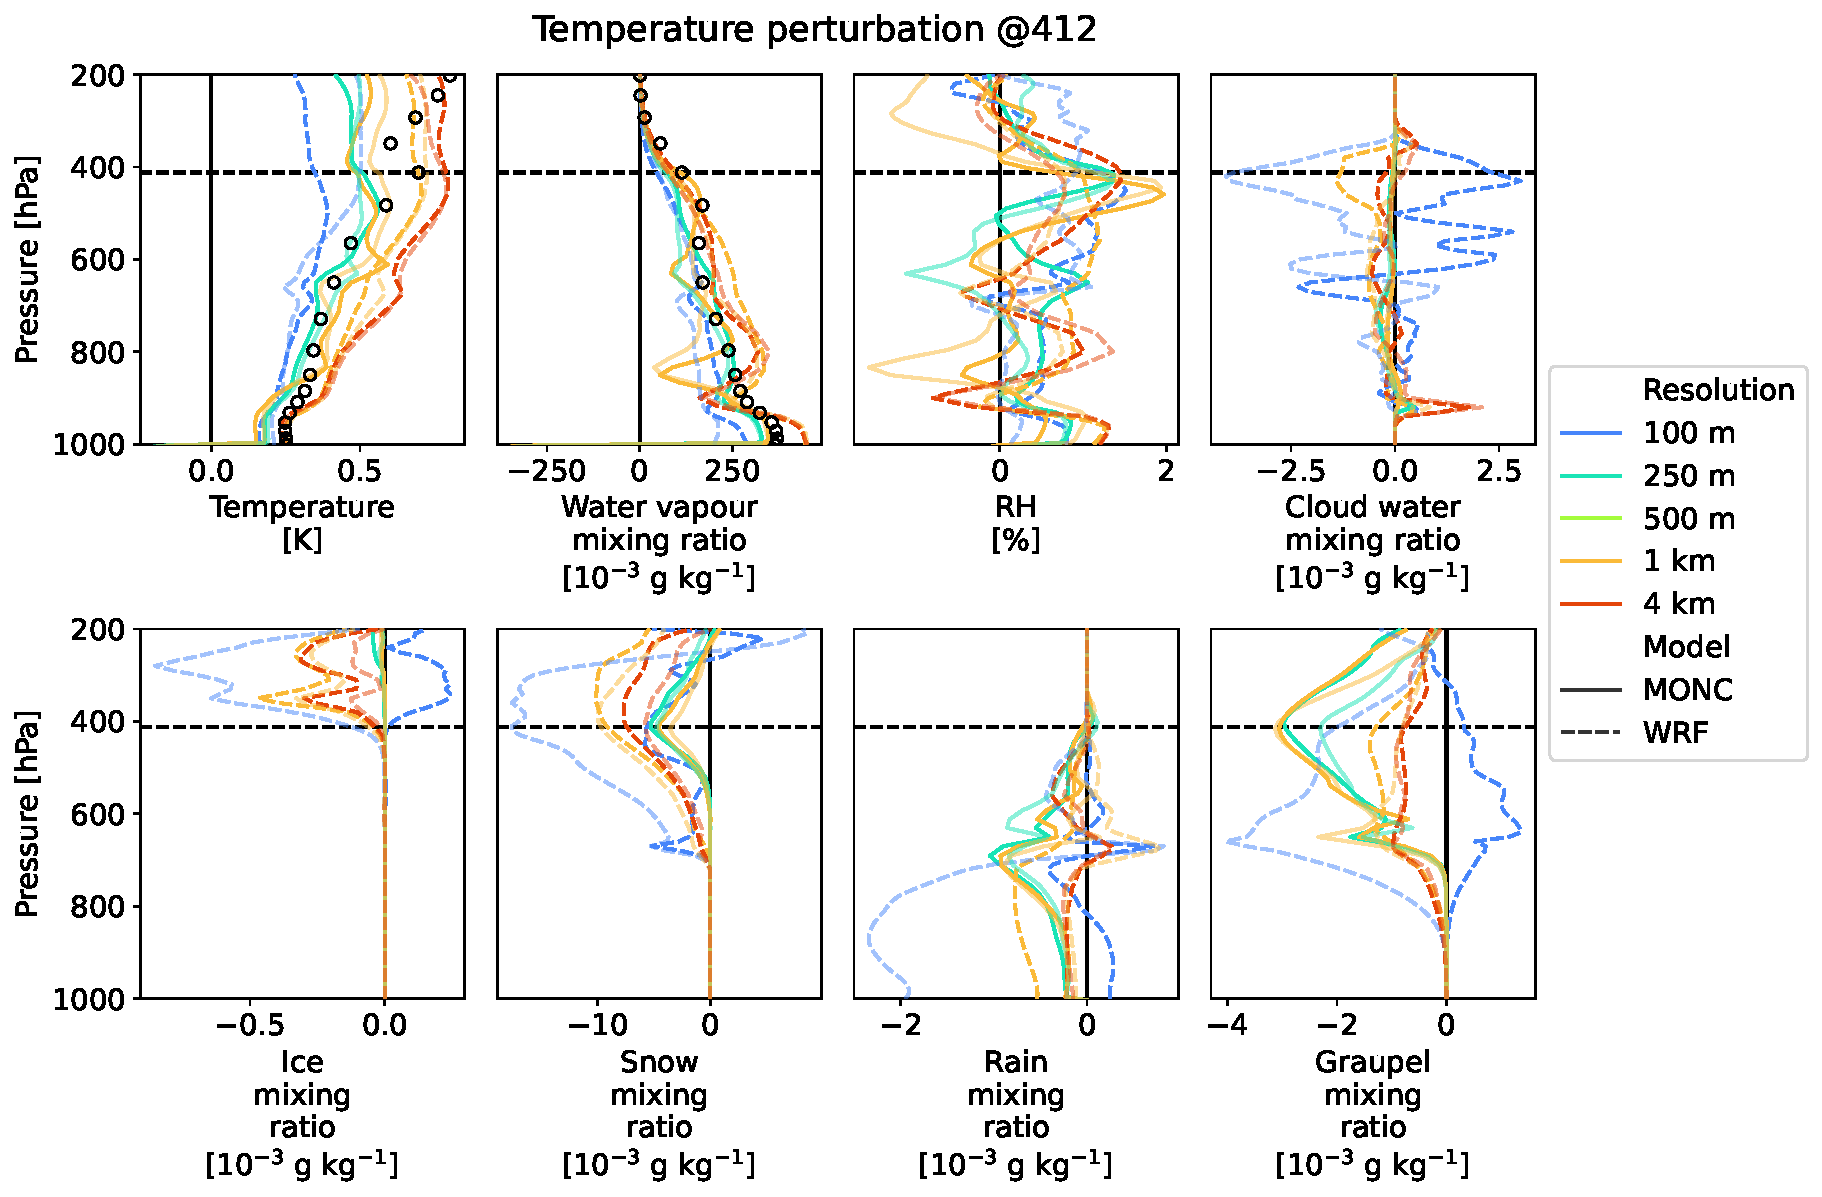
\includegraphics[width=\textwidth]{figures/pert_diffs_T_0.5_@412}
    \caption{Differences in model values by pressure, after a perturbation of
    +0.5 K was introduced in the $T$ field at 412 hPa. The solid vertical black
    line shows zero difference. The dashed horizontal line shoes the maximum
    perturbation level. MR stands for mixing ratio. Responses to positive
    perturbations are shown with opaque lines, while responses to negative
    perturbations are shown with semi-transparent lines. Responses to negative
    perturbations have been multiplied by $-1$ so they overlay responses to
    positive perturbations if the positive and negative responses are symmetric.
    Black circles show the responses to the same perturbations recorded by
    \citeA{Kuang_JAS_2010}. \todo{What's going on with WRF 100 m rain?}.
    \todo{MONC results for RH are missing in all these response plots, and
    should be added.}}
    \label{fig:tpert_412}
\end{figure}

\begin{figure}[pth]
    \noindent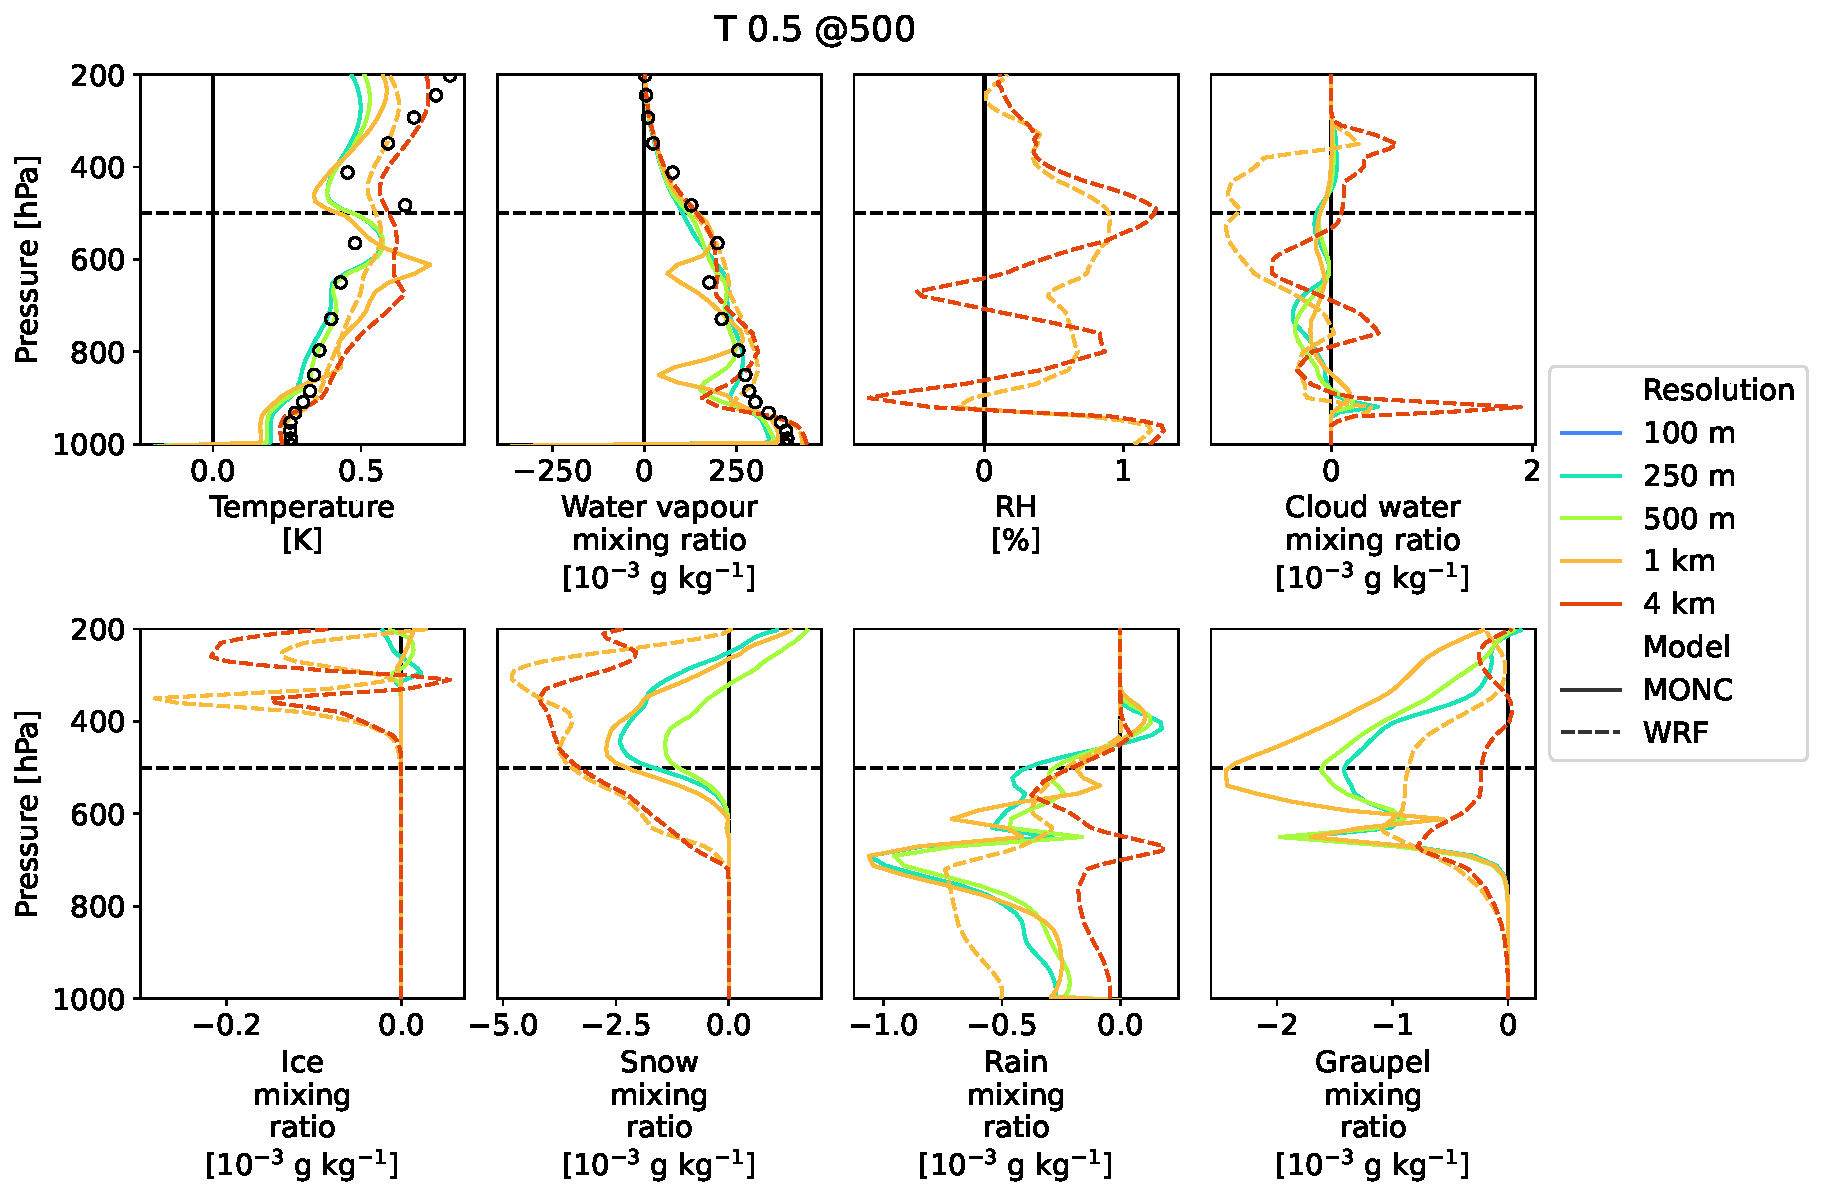
\includegraphics[width=\textwidth]{figures/pert_diffs_T_0.5_@500}
    \caption{As in Figure \ref{fig:tpert_412}, but for a perturbation at 500
    hPa, and with black circles showing the responses of \citeA{Kuang_JAS_2010}
    to a temperature perturbation at 483 hPa.}
    \label{fig:tpert_500}
\end{figure}

\begin{figure}[pth]
    \noindent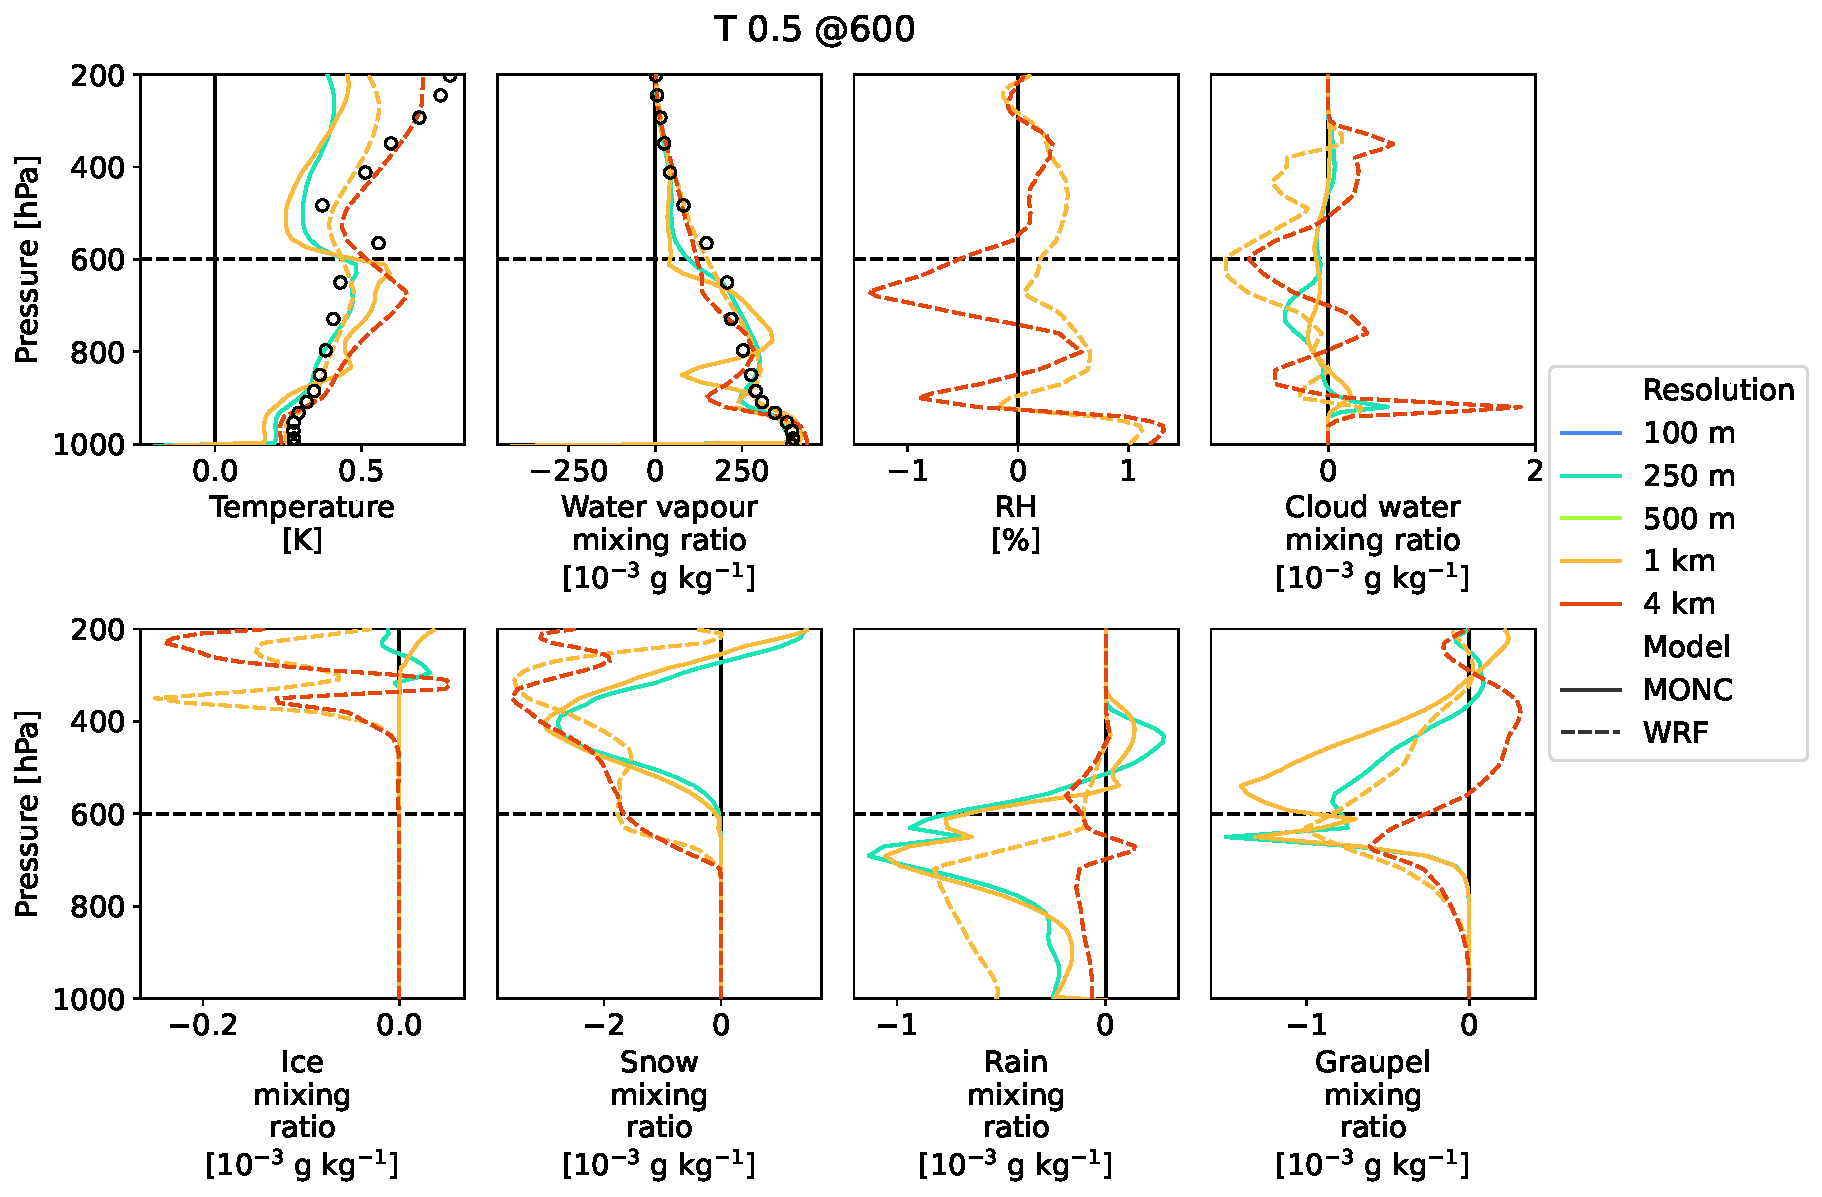
\includegraphics[width=\textwidth]{figures/pert_diffs_T_0.5_@600}
    \caption{As in Figure \ref{fig:tpert_412}, but for a perturbation at 600
    hPa, and with black circles showing the responses of \citeA{Kuang_JAS_2010}
    to a temperature perturbation at 565 hPa.}
    \label{fig:tpert_600}
\end{figure}

\begin{figure}[pth]
    \noindent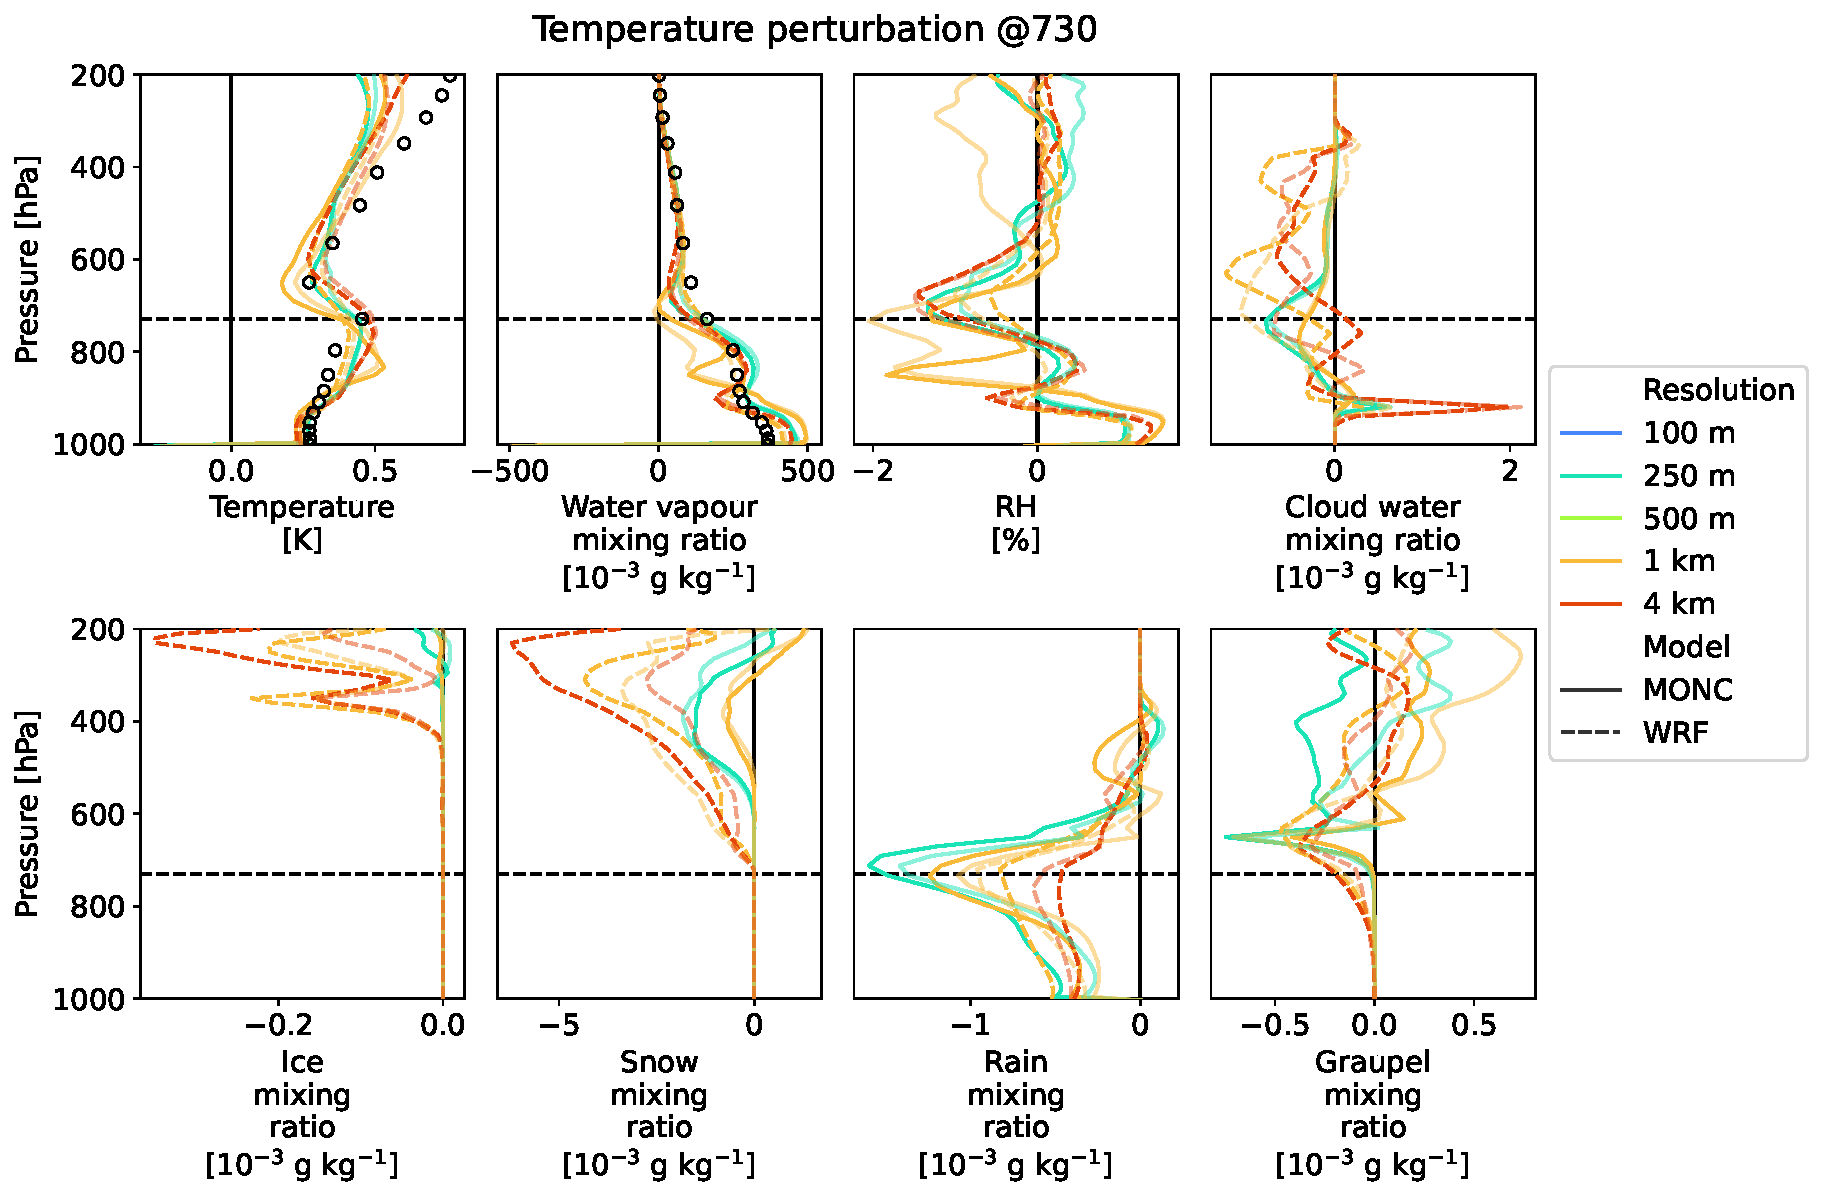
\includegraphics[width=\textwidth]{figures/pert_diffs_T_0.5_@730}
    \caption{As in Figure \ref{fig:tpert_412}, but for a perturbation at 730
    hPa, and with black circles showing the responses of \citeA{Kuang_JAS_2010}
    to a temperature perturbation at 729 hPa.}
    \label{fig:tpert_730}
\end{figure}

\begin{figure}[pth]
    \noindent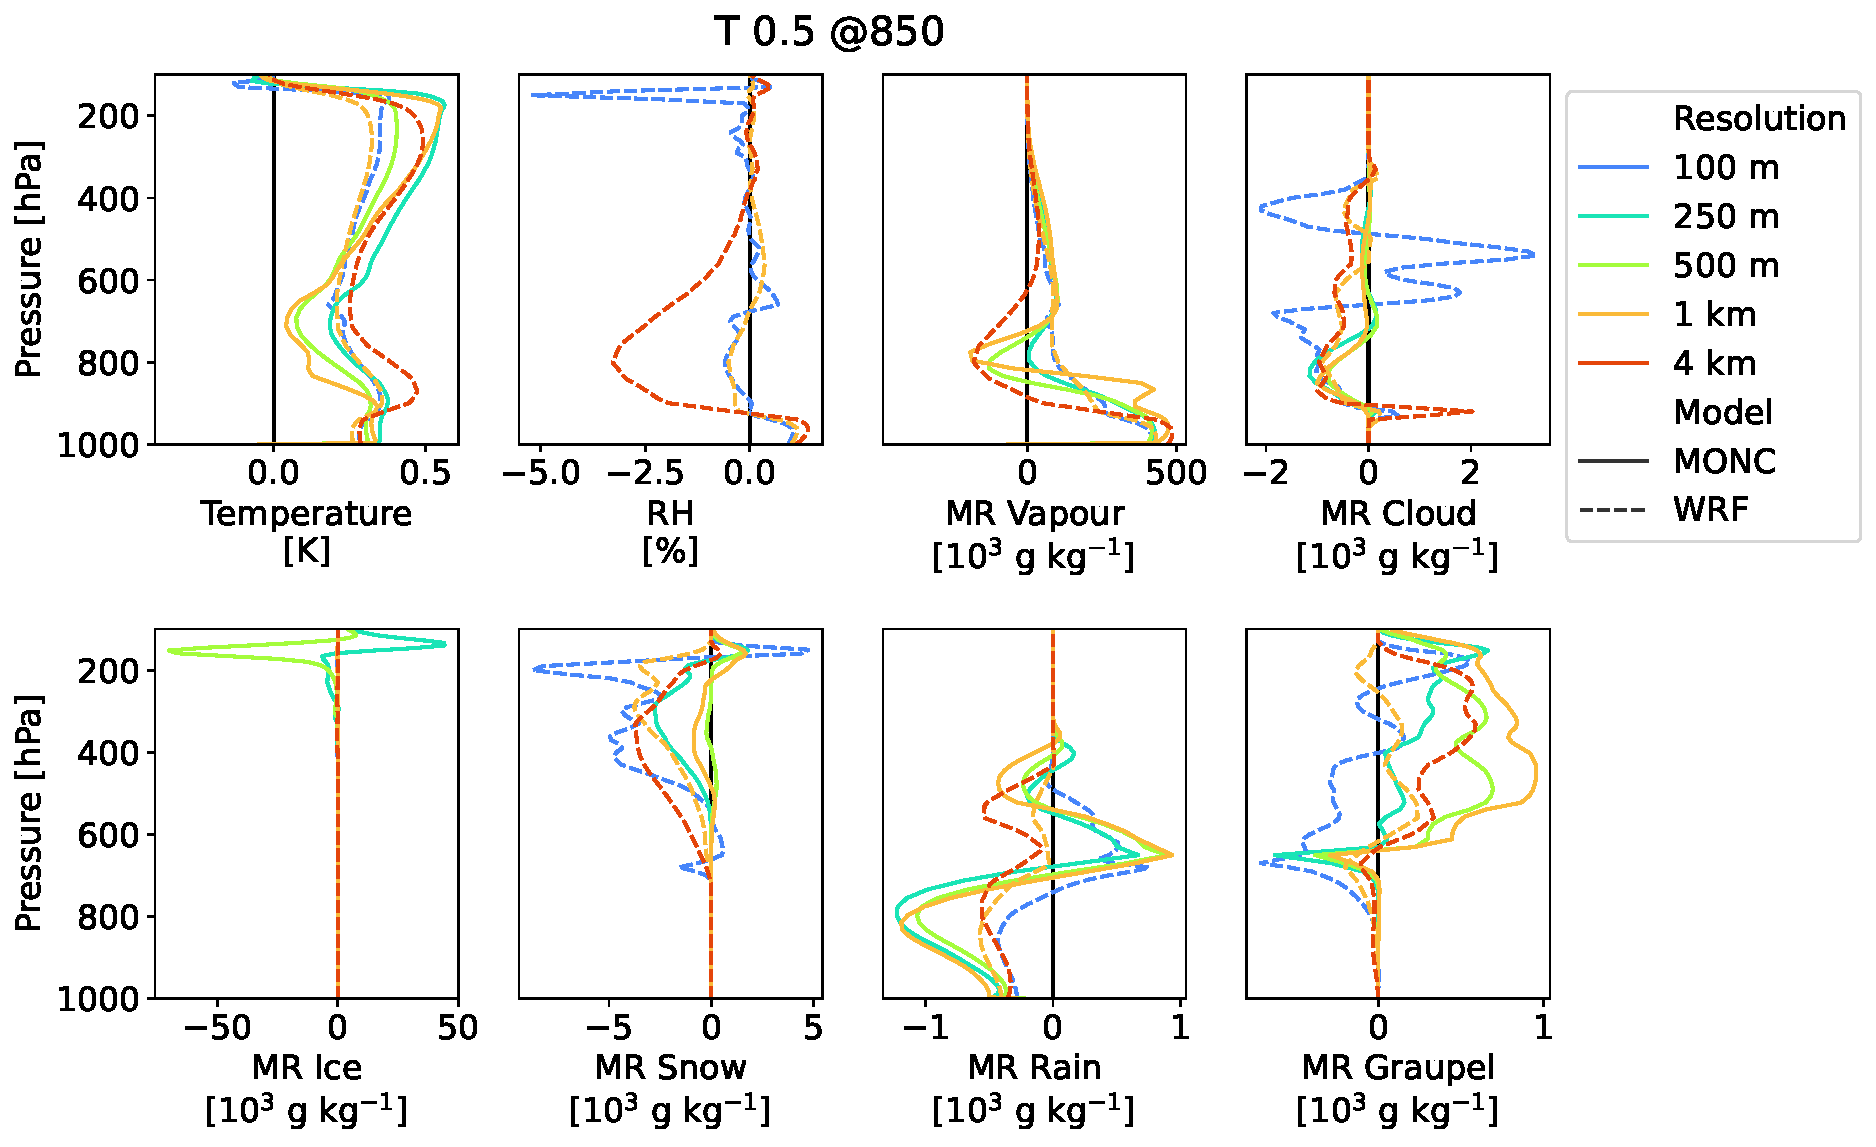
\includegraphics[width=\textwidth]{figures/pert_diffs_T_0.5_@850}
    \caption{As in Figure \ref{fig:tpert_412}, but for a perturbation at 850
    hPa, and with black circles showing the responses of \citeA{Kuang_JAS_2010}
    to a temperature perturbation at 850 hPa.}
    \label{fig:tpert_850}
\end{figure}

In response to temperature perturbations, there is a minimum in the warming in
the vicinity of the perturbation level, or just above that, and enhanced warming
below. This structure is more marked in MONC than in WRF which gives a smoother
temperature response in the vertical. The sub-km resolution runs with MONC also
produce smoother responses than the 1 km runs. In the case of the 850 hPa
perturbation the enhanced warming below is not so apparent, but there is a
relatively large warming at the surface in that case compared to responses from
the other perturbation levels.

The moisture response to the temperature perturbations is qualitatively
different at 4 km from other resolutions in WRF. A temperature perturbation at
850 hPa shows the strongest differences between the various runs. In some cases
(WRF at 4 km and MONC at 1 km and 500 m) this perturbation can induce a drying
response at and just above the perturbation level. With WRF, this response
becomes a moistening at finer resolution. With MONC, the drying is a little less
marked at 500 m rather than 1 km, and at 250 m grid spacing the response was
zero at this level. For the temperature perturbation at 850 hPa, moistening in
the boundary layer increases for coarser resolutions in WRF, and to a lesser
extent for MONC. A temperature perturbation at 412 hPa produces a minimum in the
moistening at around 900 hPa which is much more pronounced at 4 km in WRF but
still retains its sign. In MONC there is a similarly pronounced minimum seen in
the 1km run. Similar comments apply for 500 and 600 hPa as 412 hPa \todo{we do
not have runs of different resolutions for these}. There is often a small
minimum in the moistening responses around the perturbation level itself,
particularly for perturbations applied at lower levels. For a temperature
perturbation at 730 hPa, the moistening minimum around the application level is
pronounced in MONC and reaches around zero, but it does not produce the drying
seen when the perturbation is applied at 850 hPa. One way to think about the
drying with perturbations at 850 hPa is that the minimum we see consistently
just above the boundary layer combines with the minimum that we consistently see
at the perturbation level.

We now turn to the responses in hydrometeor content to perturbations in the
temperature field. For the temperature perturbation at 850 hPa in WRF, there is
a reduction of rain below the freezing level. A reduction in cloud liquid water
also occurs, and this is over a deeper layer in WRF than in MONC. There is also
some reduction to snow and increase in graupel at upper levels. Changes of
broadly similar character occur in the hydrometeor responses to the other
temperature perturbations in WRF, except that the profiles of liquid water
changes have reductions with minima that are aligned with or just above the
perturbation height. The responses of hydrometeors in MONC have a broadly
similar character, but some of the amplitudes are quite different. There are
similar amplitudes to WRF for rain, but weaker responses in liquid water, ice
and snow. MONC responded more strongly for graupel, however, especially in
response to perturbations at 412 and 500 hPa. For the temperature perturbation
at 850 hPa in MONC, rain has a stronger reduction than in WRF below the freezing
level but is increased around the freezing level, which is a feature not seen in
the WRF results except in the 100 m grid spacing run. The cloud liquid water is
reduced similarly to WRF at low levels but the reductions are more confined, not
extending to the same heights. In MONC, for the response to the temperature
perturbation at 850 hPa, there are some nonlinear changes with grid length. For
example, the rain and liquid water reductions at low levels are weaker at 500 m
but stronger at 250 m.  Snow is also more strongly reduced at 500 m than at 1 km
but there is barely any reduction at 250m. The increase in graupel becomes
weaker with increasing resolution. For MONC with the 730 hPa perturbation, there
was no \todo{500 m} grid spacing simulation but the comments above also apply
for the qualitative changes between 1 km and \todo{250 m} grid spacings. For the
600 hPa perturbation, there was no \todo{500 m} MONC simulation and there is
very little difference in the hydrometeor response between 1km and \todo{250 m}.

\subsection{Responses to Perturbations in Moisture}

The responses of the models to perturbations in moisture at 412 hPa, 500 hPa,
600 hPa, 730 hPa, and 850 hPa are shown in Figures \ref{fig:qpert_412},
\ref{fig:qpert_500}, \ref{fig:qpert_600}, \ref{fig:qpert_730}, and
\ref{fig:qpert_850}, respectively. Several elements of these results are similar
to the results for temperature perturbations: moisture and hydrometeor responses
to moisture perturbations are smaller than the changes in the mean profiles due
to resolution, WRF and MONC produced responses of similar amplitude, except for
cloud liquid water and ice where the changes in MONC were much smaller, and
again MONC is more likely to show nonlinearity to positive and negative
perturbations than WRF \todo{Not sure this is true when looking at e.g. the 730
results for WRF RH or the 412 hPa results for cloud water or rain at 100 m}. In
this case the strongest example of nonlinearity in MONC is the temperature
response in the mid levels to a moisture perturbation at 600 hPa.

\begin{figure}[pth]
    \noindent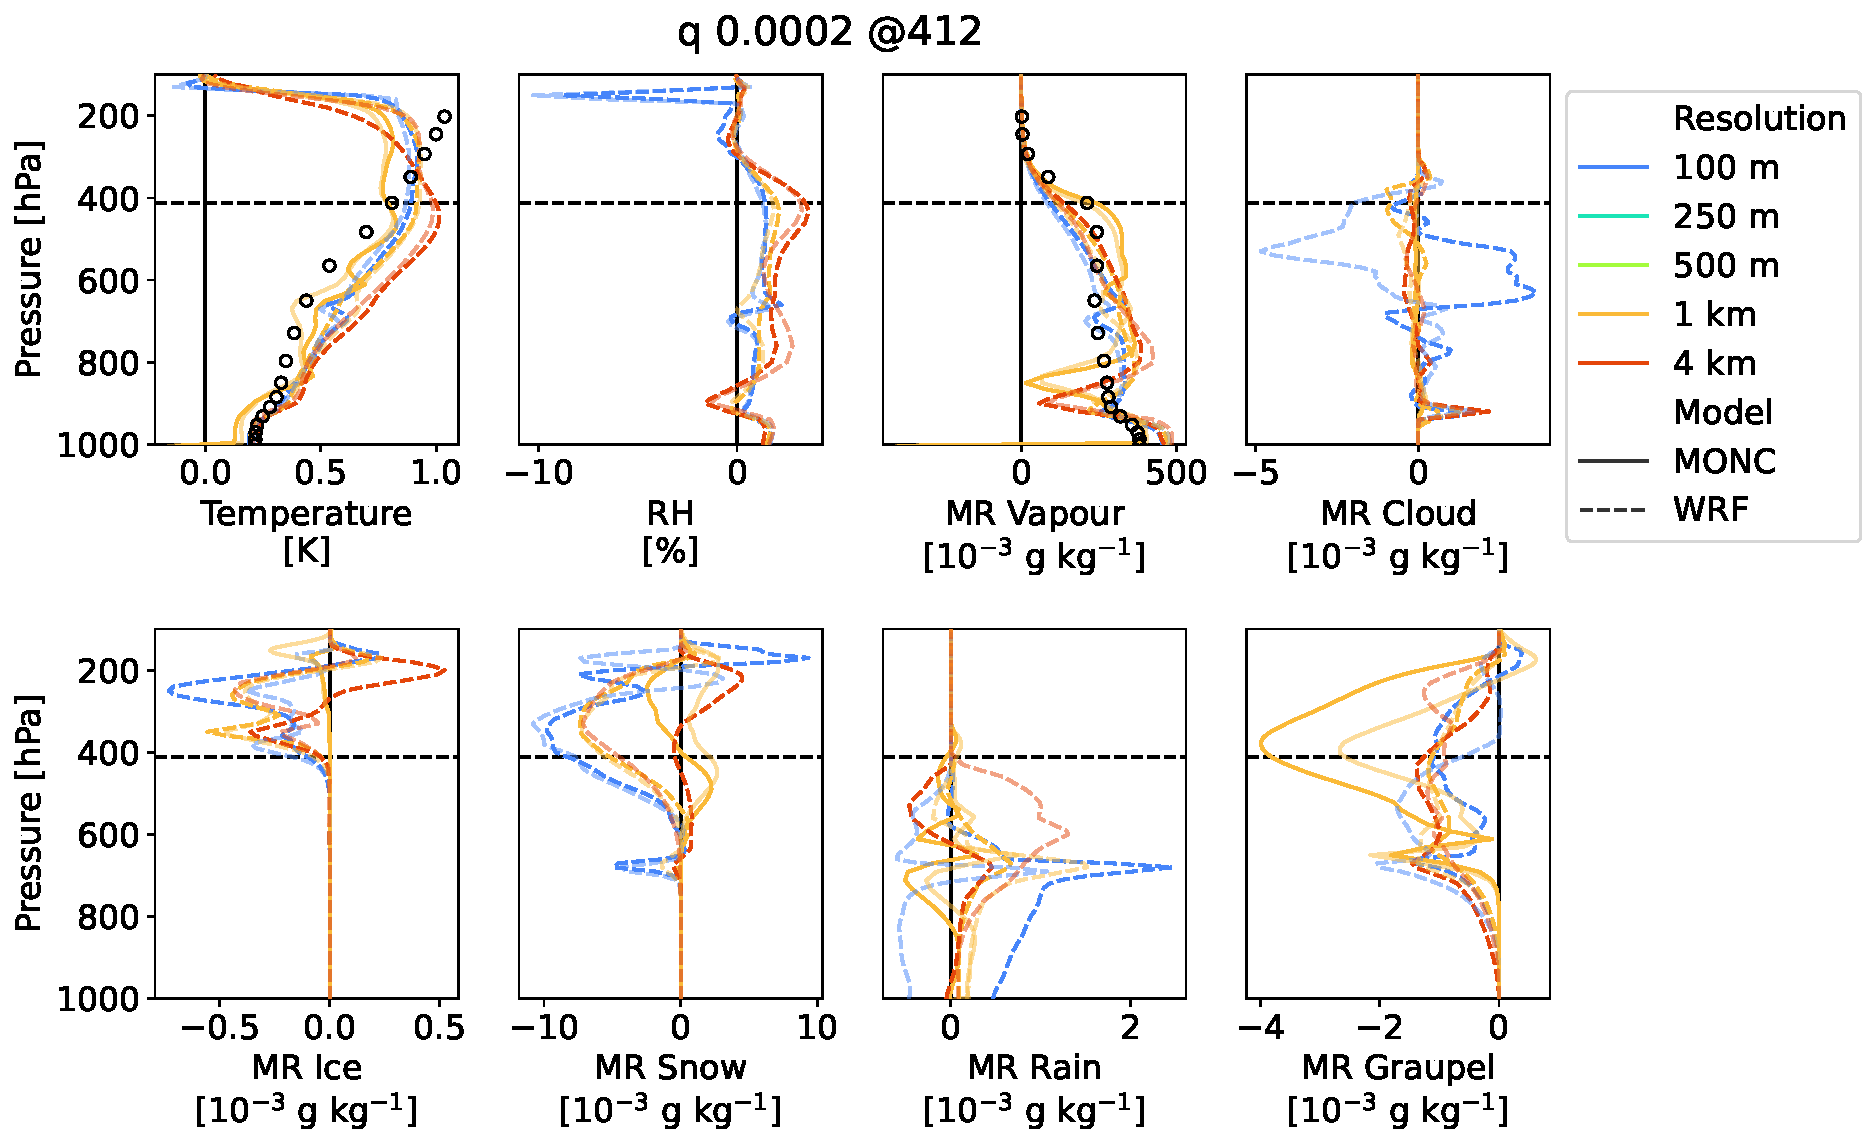
\includegraphics[width=\textwidth]{figures/pert_diffs_q_0.0002_@412}
    \caption{Differences in model values by pressure, after a perturbation of
    0.2 g kg$^{-1}$ was introduced in the $q$ field at 412 hPa. The solid
    vertical black line shows zero difference. The dashed horizontal line shoes
    the maximum perturbation level. MR stands for mixing ratio. Responses to
    positive perturbations are shown with opaque lines, while responses to
    negative perturbations are shown with semi-transparent lines. Responses to
    negative perturbations have been multiplied by $-1$ so they overlay
    responses to positive perturbations if the positive and negative responses
    are symmetric. Black circles show the responses to the same perturbations
    recorded by \citeA{Kuang_JAS_2010}. \todo{What's going on with WRF 100 m
    rain?}. \todo{MONC results for RH are missing in all these response plots,
    and should be added.}}
    \label{fig:qpert_412}
\end{figure}

\begin{figure}[pth]
    \noindent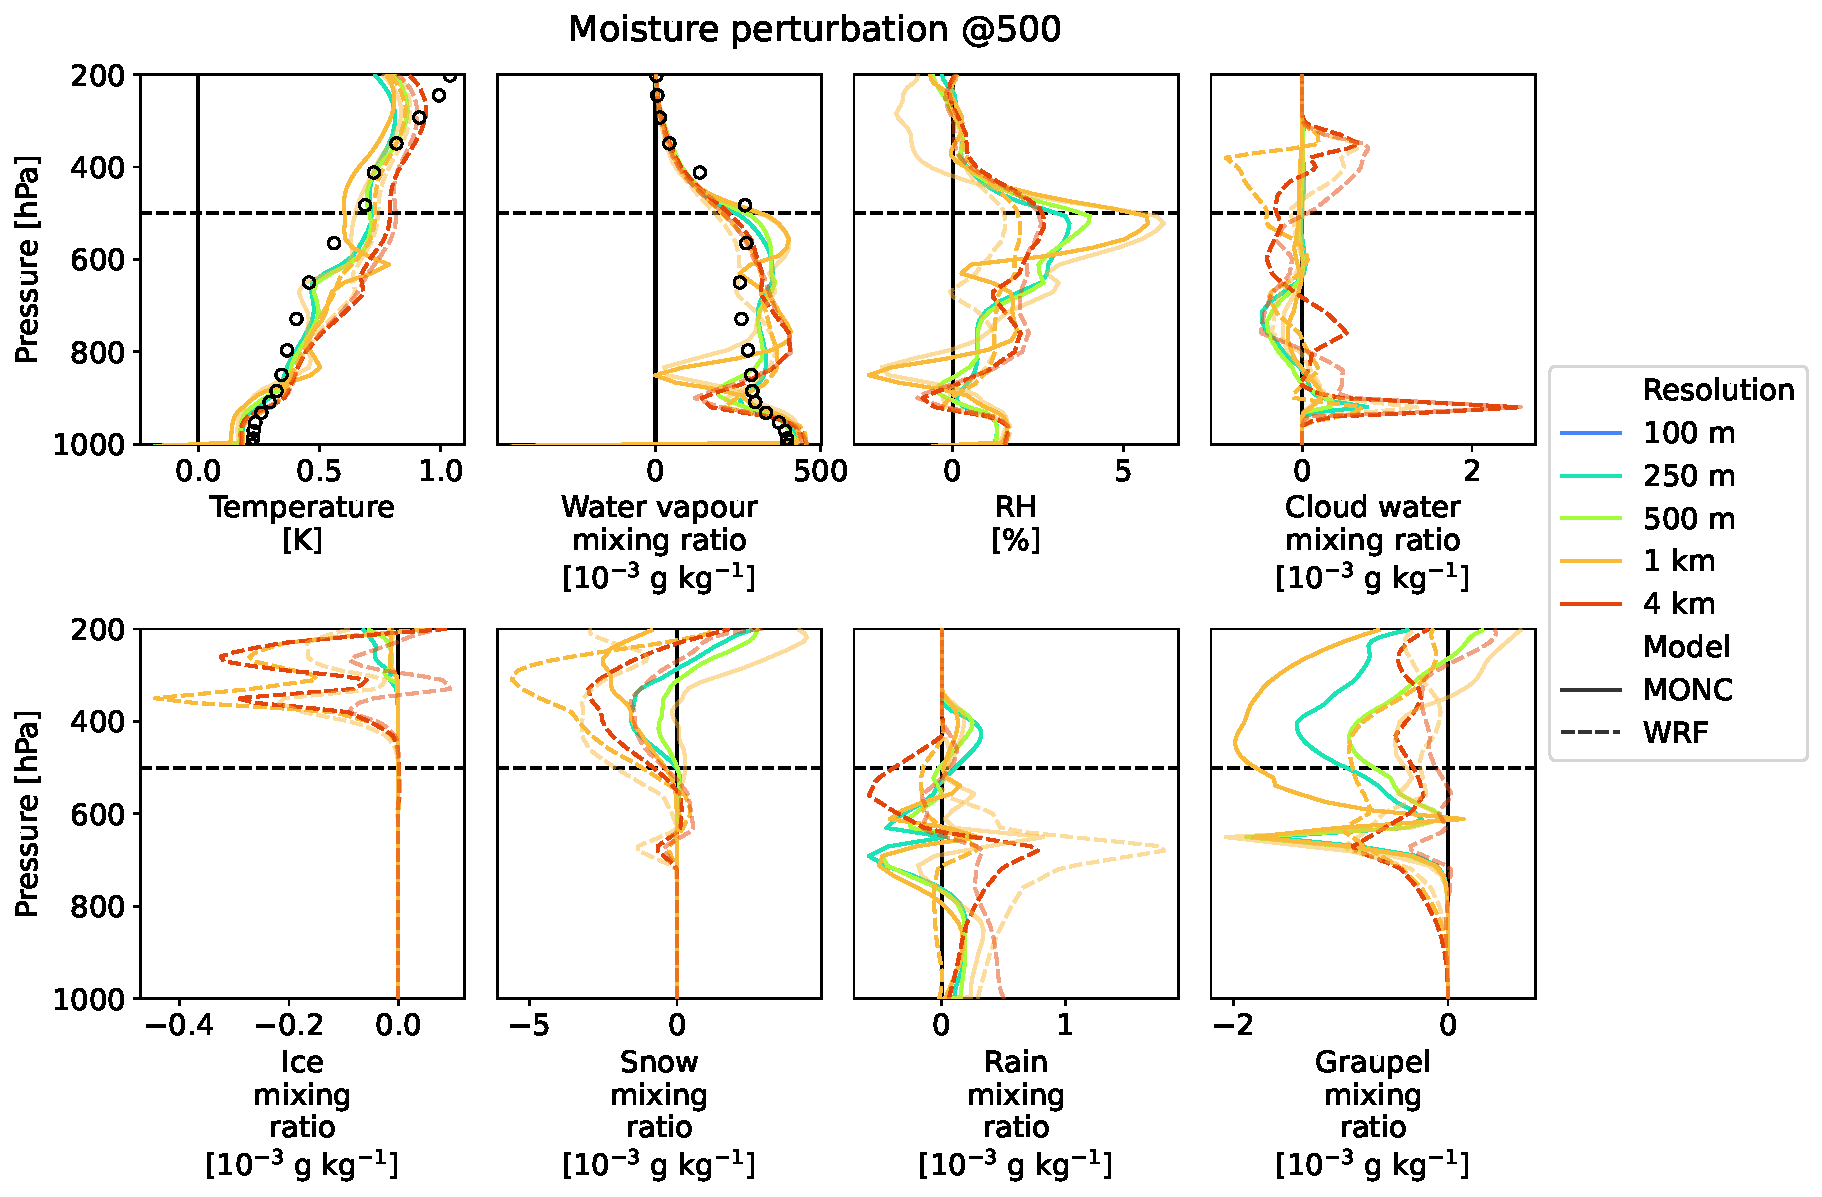
\includegraphics[width=\textwidth]{figures/pert_diffs_q_0.0002_@500}
    \caption{As in Figure \ref{fig:qpert_412}, but for a perturbation at 500
    hPa, and with black circles showing the responses of \citeA{Kuang_JAS_2010}
    to a temperature perturbation at 483 hPa.}
    \label{fig:qpert_500}
\end{figure}

\begin{figure}[pth]
    \noindent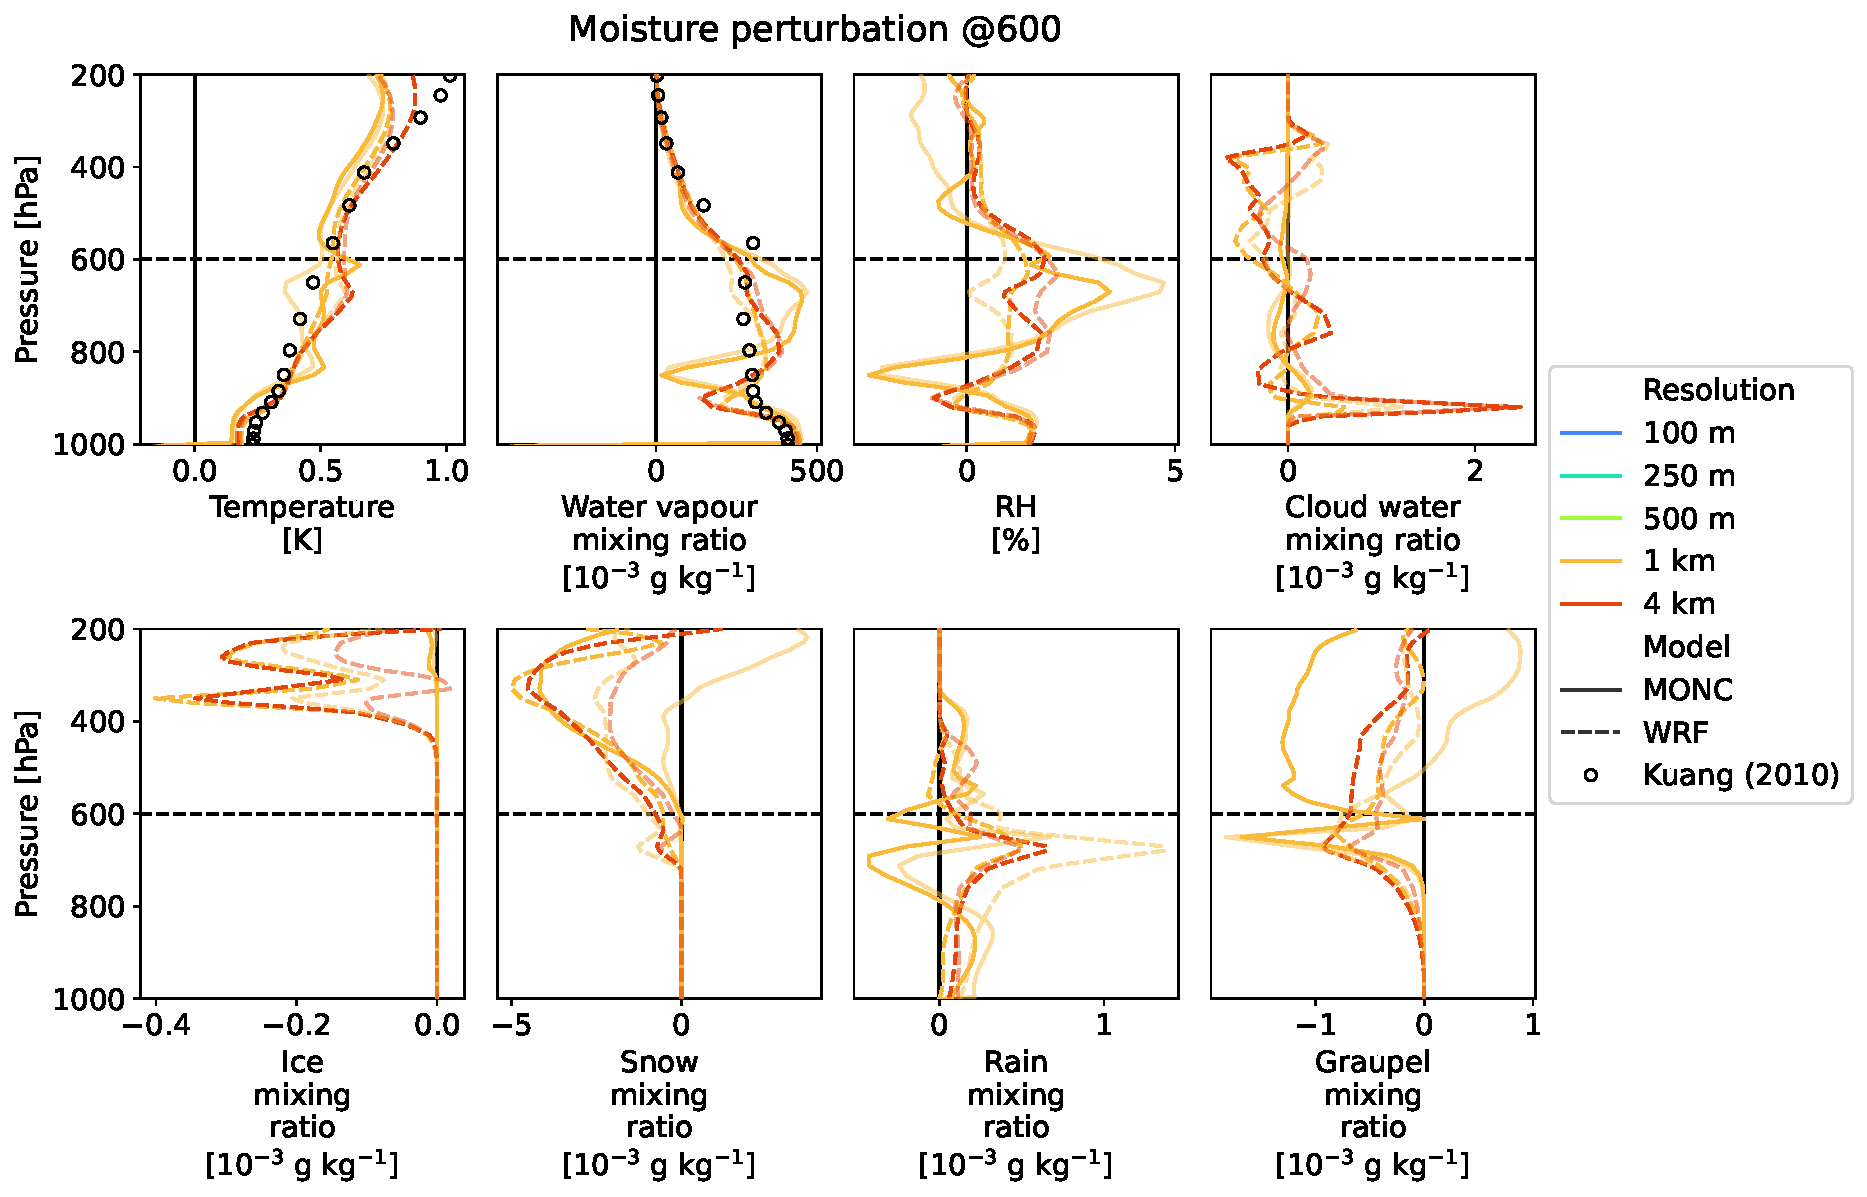
\includegraphics[width=\textwidth]{figures/pert_diffs_q_0.0002_@600}
    \caption{As in Figure \ref{fig:qpert_412}, but for a perturbation at 600
    hPa, and with black circles showing the responses of \citeA{Kuang_JAS_2010}
    to a temperature perturbation at 565 hPa.}
    \label{fig:qpert_600}
\end{figure}

\begin{figure}[pth]
    \noindent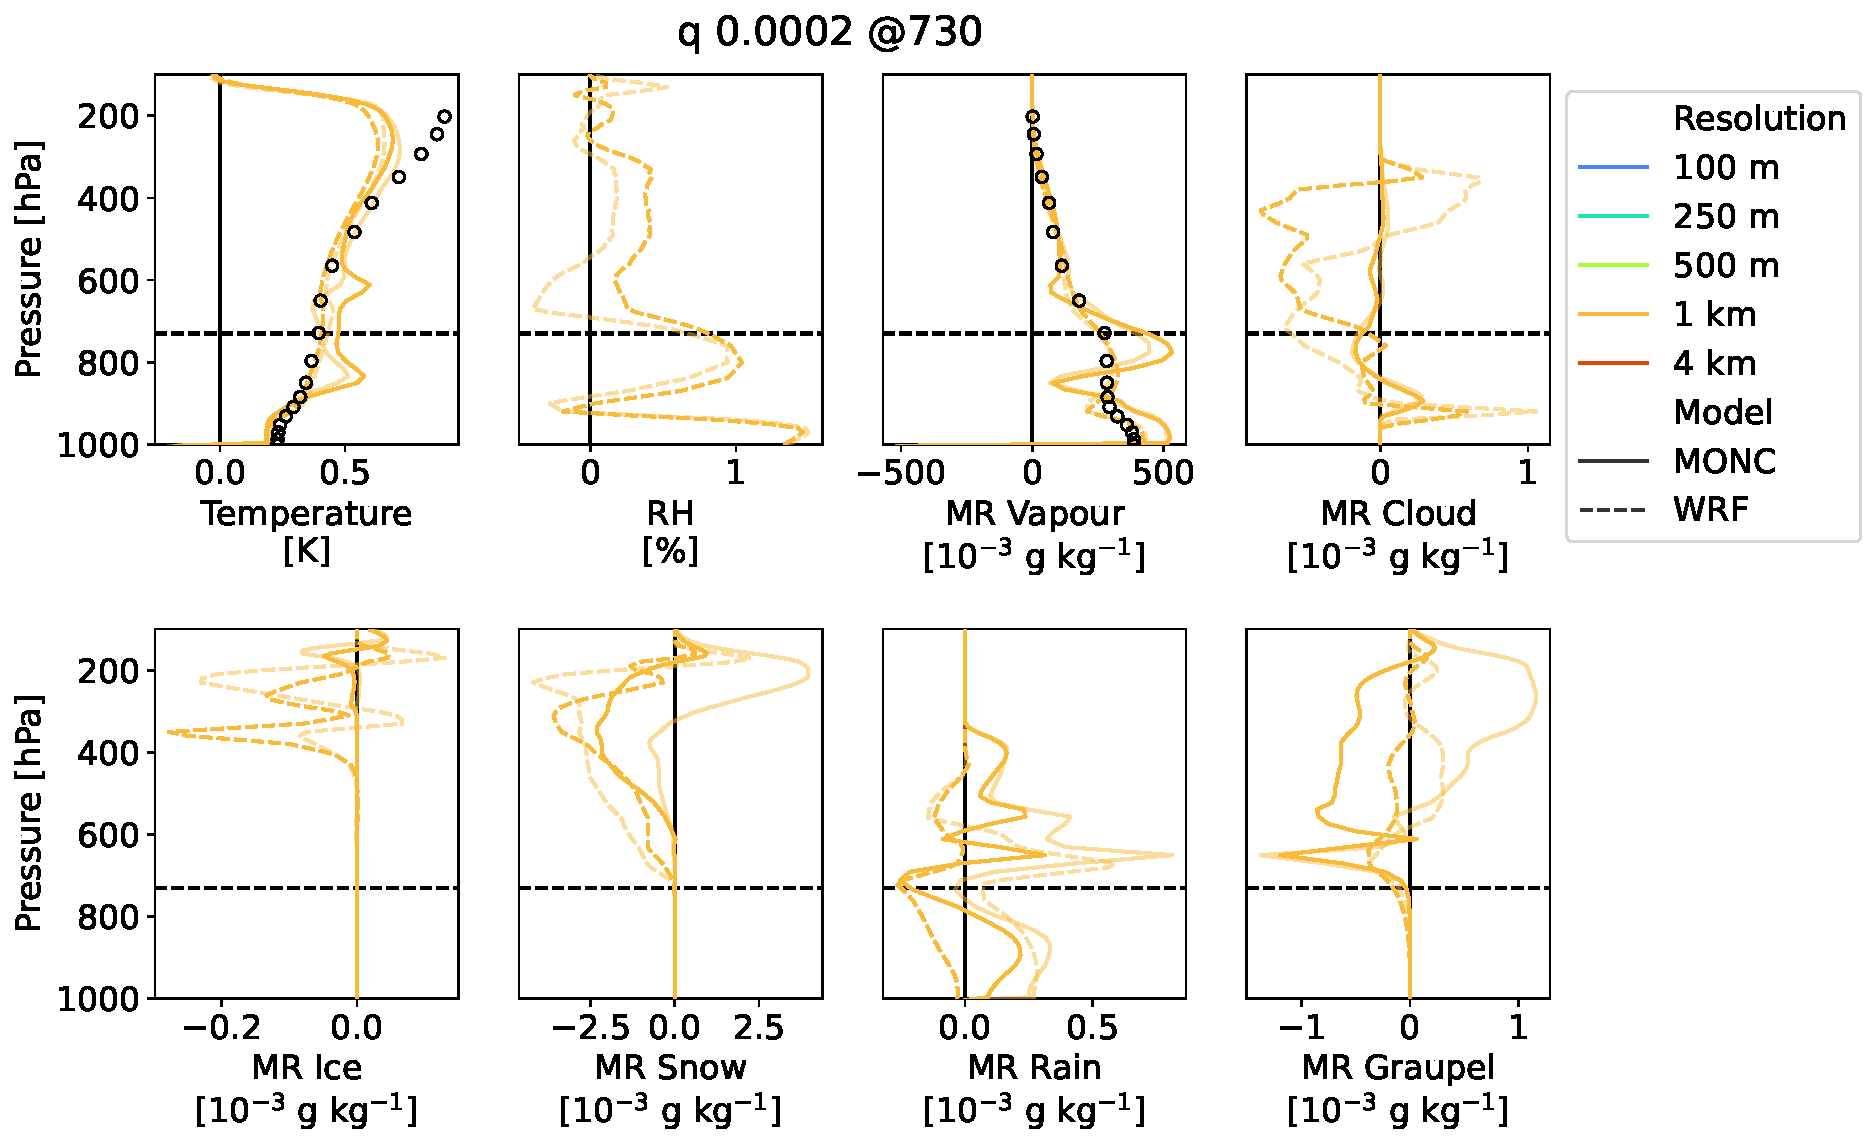
\includegraphics[width=\textwidth]{figures/pert_diffs_q_0.0002_@730}
    \caption{As in Figure \ref{fig:qpert_412}, but for a perturbation at 730
    hPa, and with black circles showing the responses of \citeA{Kuang_JAS_2010}
    to a temperature perturbation at 729 hPa.}
    \label{fig:qpert_730}
\end{figure}

\begin{figure}[pth]
    \noindent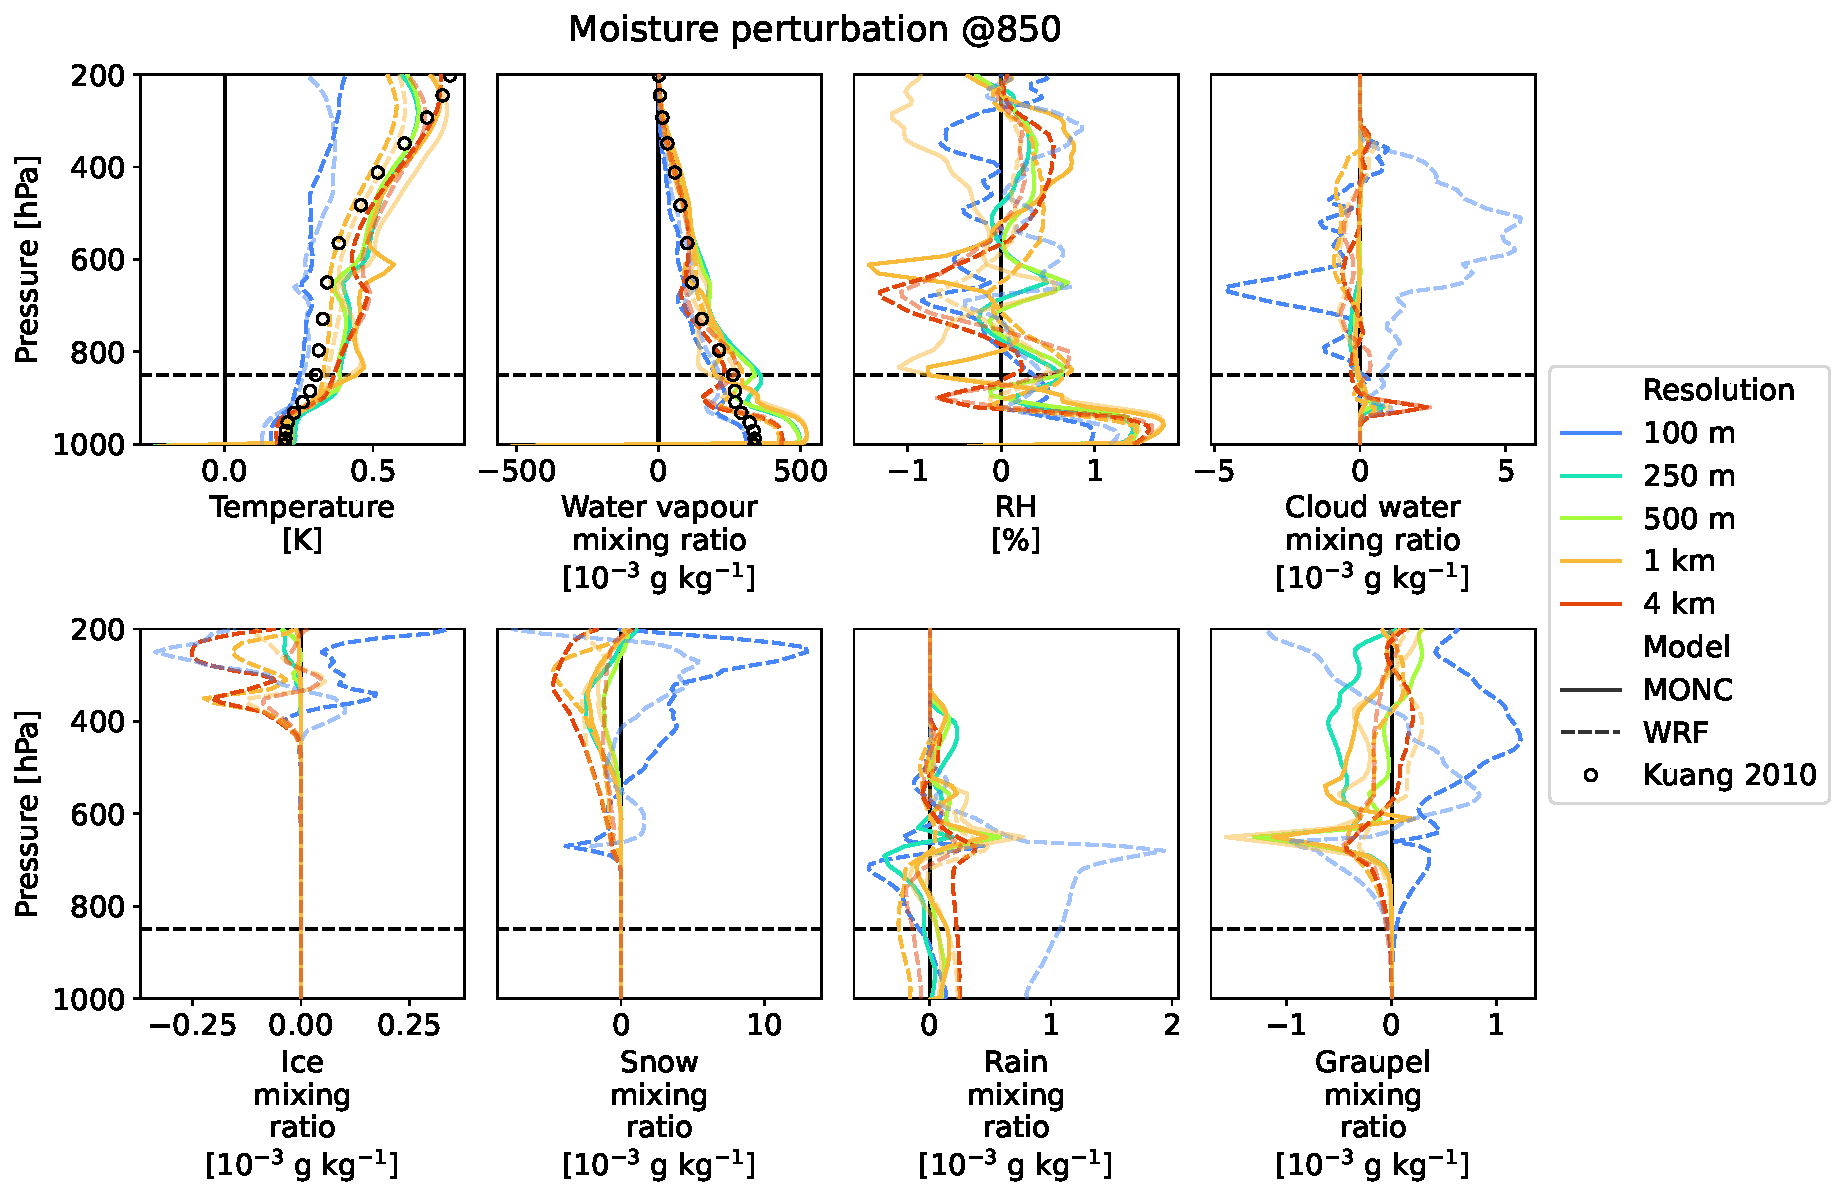
\includegraphics[width=\textwidth]{figures/pert_diffs_q_0.0002_@850}
    \caption{As in Figure \ref{fig:qpert_412}, but for a perturbation at 850
    hPa, and with black circles showing the responses of \citeA{Kuang_JAS_2010}
    to a temperature perturbation at 850 hPa.}
    \label{fig:qpert_850}
\end{figure}

We first examine responses to temperature profiles in response to moisture
perturbations. Warming in the boundary layer is very consistent between
resolutions in WRF, but the free tropospheric warming is stronger at coarser
resolution. Particularly notable is the increase between 500 m and 1 km grid
spacings for a perturbation at 412 hPa. The boundary layer warming is also very
consistent between WRF and MONC. The free tropospheric warming is stronger in
MONC for a low-level moisture perturbation and weaker for an upper-level
moisture perturbation.

In response to moisture perturbations, the response in moisture fields in WRF
has minima at around 900 hPa and to a lesser extent around 650 hPa. These minema
are modest at fine grid spacing but at coarse resolution, the lower minimum
becomes much stronger, even for perturbations made at upper levels. It does
however remain a moistening response. Such minima are also present in MONC, the
lower level one being a little higher and much more pronounced than in WRF at
the same grid spacings. This is somewhat reminiscent of the 1 km WRF simulation,
and again, remains as a moistening response. \todo{Bob: It would be interesting
to compare this with a higher resolution MONC run, but we mainly focussed extra
runs on temperature perturbations I'm not sure if we currently have that
available for moisture perturbations.} Moistening in the boundary layer is
weaker at 500m than at coarser resolutions in WRF. While the responses across
most of the vertical profile are symmetric with positive and negative
perturbations, in WRF the moisture responses are often non-symmetric around the
650 hPa minimum.

We now examine the hydrometeor responses to moisture perturbations. For the
moisture perturbation at 850 hPa in WRF, there is a nonlinearity in the sign of
the rain response below the freezing level at about 1 km. There is a consistent
reduction in cloud liquid water, ice and snow, with the exception of the 100 m
grid spacing runs in which a non-linearity shows cloud-water increases between
400 hPa and 600 hPa for a positive moisture perturbation. Graupel is
consistently reduced around 600 hPa but there are responses with opposite signs
in the upper levels. Changes of broadly similar character occur in the
hydrometeor responses in WRF to the other moisture perturbations. The rain water
changes to being a consistent increase for the 412 hPa and 500 hPa perturbations
with a spike at the freezing level. The cloud liquid water responses have
complex shapes for higher level perturbations with the main responses more
towards the upper levels. Graupel is consistently reduced for perturbations at
and above 600 hPa. The responses of hydrometeors in MONC are generally weaker
for liquid water, ice and snow. MONC responds more strongly for graupel,
however, especially in response to higher level perturbations where
non-linearities are evident. For the 850 hPa moisture perturbation in MONC, rain
increases below freezing level and around the freezing level, in contrast with
most of the WRF results. The cloud liquid water is \todo{slightly increased?} at
low levels only. Snow and ice are reduced, as is graupel. Changes of broadly
similar character occur in the hydrometeor responses to the other moisture
perturbations in MONC. The exception is for graupel which has some large and
non-linear responses in response to higher level perturbations. 

\section{Conclusions}
\label{sec:conclusions}

%% Enter Figures and Tables near as possible to where they are first mentioned:
%
% DO NOT USE \psfrag or \subfigure commands.
%
% Figure captions go below the figure.
% Table titles go above tables;  other caption information
%  should be placed in last line of the table, using
% \multicolumn2l{$^a$ This is a table note.}

% \begin{figure}
% \noindent\includegraphics[width=\textwidth]{anothersample.png}
% \caption{caption}
% \label{pngfiguresample}
% \end{figure}

% Acronyms
%  \begin{acronyms}
%  \acro{Acronym}
%  Definition here
%  \acro{EMOS}
%  Ensemble model output statistics
%  \acro{ECMWF}
%  Centre for Medium-Range Weather Forecasts
%  \end{acronyms}

\section{Open Research}

% AGU requires an Availability Statement for the underlying data needed to
% understand, evaluate, and build upon the reported research at the time of peer
% review and publication.

% Authors should include an Availability Statement for the software that has a
% significant impact on the research. Details and templates are in the
% Availability Statement section of the Data and Software for Authors Guidance:
% \url{https://www.agu.org/Publish-with-AGU/Publish/Author-Resources/Data-and-Software-for-Authors#availability}

% It is important to cite individual datasets in this section and, and they must
% be included in your bibliography. Please use the type field in your bibtex file
% to specify the type of data cited. Options include [Dataset], [Software],
% [ComputationalNotebook], [Collection].
% Example:
%
%@misc{https://doi.org/10.7283/633e-1497,
%  doi = {10.7283/633E-1497},
%  url = {https://www.unavco.org/data/doi/10.7283/633E-1497},
%  author = {de Zeeuw-van Dalfsen, Elske and Sleeman, Reinoud},
%  title = {KNMI Dutch Antilles GPS Network - SAB1-St_Johns_Saba_NA P.S.},
%  publisher = {UNAVCO, Inc.},
%  year = {2019},
%  type = {dataset}
%}

\bibliography{library}
\end{document}
